
\chapter{Construction}
 
 {\slshape \scshape ``The first little pig was very lazy. He didn't want to work at all and he built his house out of straw. The second little pig worked a little bit harder but he was somewhat lazy too and he built his house out of sticks. The third little pig worked hard all day and built his house with bricks. It looked like it could withstand the strongest winds." - English Folk Tale}
 
 The parable of the three little pigs reminds us that how we build things is important. And while at first blush, the story seems to be about how you should always build strong out of brick, sometimes we should learn from the first pig, and build fast for prototyping. Having a suite of different fabrication techniques at hand can be incredibly handy.
 
 \section{Materials}
 
 Everything is made from materials. There are a lot of different materials out there, all with different properties. Some are natural and some are completely synthetic, but all can be measured, quantified, and compared. Important properties we'll focus on are:
 
 \begin{compactitem}
 	\item Density (weight)
 	\item Stiffness
 	\item Hardness
 	\item Strength
 	\item Toughness
 	\item Thermal capabilities
 	\item Frictional and chemical interactions
 \end{compactitem}
 
 You'll notice that stiffness, strength, hardness, and toughness are all different characteristics. They are distinctly different properties in engineering.
 
 \subsection{Stress-Strain Properties}
 \index{stress-strain behavior}
 To show this, we'll first consider a \textit{stress-strain curve}. This curve is created by pulling on a specimen of material like shown, interpreting the force and deflection data into \textit{stress} $\sigma$ (force per cross-sectional area) and \textit{strain} $\epsilon$ (percent deflection).
 
 \begin{figure}[H]
 \begin{subfigure}[]{.4\linewidth}
 	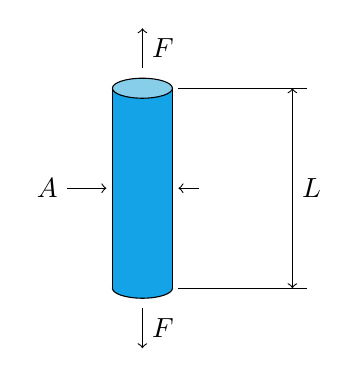
\begin{tikzpicture}[x=1.5in, y=1.0in]
 	\filldraw[fill=Cerulean] (0,0) ellipse (0.1 and 0.05);
 	\fill[Cerulean] (-0.1,0)--(-0.1,1)--(0.1,1)--(0.1,0)--cycle;
 	 	\filldraw[fill=SkyBlue] (0,1) ellipse (0.1 and 0.05);
 	
 		\draw[ ] (-0.1,0) -- (-0.1, 1);
 		\draw[ ] (0.1,0) -- (0.1, 1);
 		\draw[->] (0,-0.1)--(0,-0.3) node[pos=0.5, right]{$F$};
 		\draw[->] (0,1.1)--(0,1.3) node[pos=0.5, right]{$F$};
 		
 		\draw[->] (-0.25,0.5)--(-0.12,0.5) node[pos=0, left]{$A$};
 		\draw[->] (0.19,0.5)--(0.12,0.5);
 		
 		\draw[<->] (0.5,0)--(0.5,1) node[pos=0.5, right]{$L$};
 		\draw[] (0.12,0)--(0.55,0); \draw[] (0.12,1)--(0.55,1);
 	\end{tikzpicture}
 \end{subfigure}\begin{subfigure}[]{.4\linewidth}
	\vspace*{\fill}
	\Large
  	\begin{align}
 		\sigma &= \frac{F}{A} \\
 		 \nonumber \\
 		\epsilon &= \frac{\Delta L}{L}
 	\end{align}
 	\vspace*{\fill}
 	\end{subfigure}
 \caption{Stress-strain test, and the relationship between the variables.}
\end{figure}
 
 \begin{figure}[H]
 	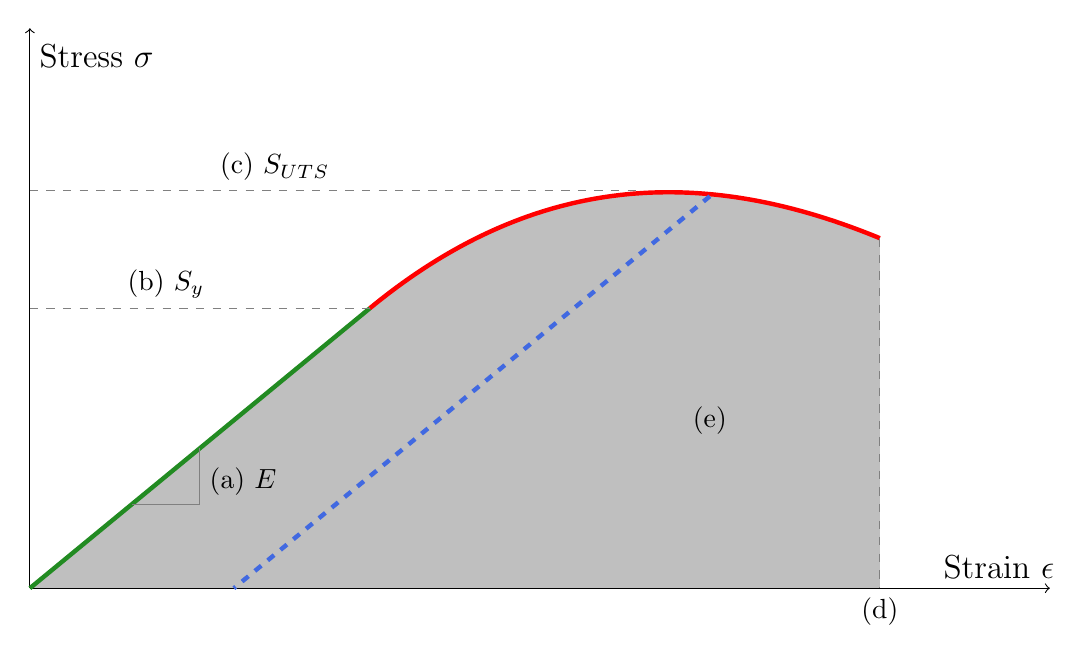
\begin{tikzpicture}[x=1.7in, y=1.4in]
		\fill[lightgray]  (0,0) -- (1,1) .. controls (1.5,1.5) and (2.0,1.5) .. (2.5,1.25) -- (2.5,0) -- cycle;	
 	
 		\draw[->] (0,0)--(3,0) node[pos=0.95, above]{\large Strain $\epsilon$};
 		\draw[->] (0,0)--(0,2) node[pos=0.95, right]{\large Stress $\sigma$};
 		\draw[ForestGreen, ultra thick] (0,0)--(1,1);
 		\draw[gray, dashed] (0,1)--(1,1) node[pos=0.4, above, black]{(b) $S_{y}$};
 		\draw[gray, dashed] (0,1.42)--(1.8,1.42) node[pos=0.4, above, black]{(c) $S_{UTS}$};
 		\draw[gray] (0.3,0.3)--(0.5,0.3)--(0.5,0.5) node[pos=0.4, right, black]{(a) $E$};
  		%\draw[gray] (1,1)--(1.8,1.8);
 		\draw[Red, ultra thick]  (1,1) .. controls (1.5,1.5) and (2.0,1.5) .. (2.5,1.25);
 		\draw[RoyalBlue, ultra thick, dashed] (2,1.4)--(0.6,0);
 		\draw[gray, dashed] (2.5,1.25)--(2.5,0) node[pos=1, below, black]{(d)};
 		
 		\node[black] at (2,0.6){(e)};
 	\end{tikzpicture}
 	\caption{Exemplary stress-strain behavior.}
 \end{figure}
 \index{stress-strain behavior!elasticity and plasticity}
 The portion of the curve that is linear (highlighted in green) is referred to as the \textit{elastic} portion. When the material is operating in this region, it will always snap back, like a rubber band. If, however, we dip into the \textit{plastic} portion of the curve (highlighted in red), when we release the material, it will have permanently deformed (following the diagonal blue dashed line).
 
 The key aspects of the curve can be boiled down into a few properties.
 
 \begin{asparaenum}[a)]
 	\item \textit{Young's Modulus}, or the \textit{Elastic Modulus} ($E$) is the slope of the elastic portion of the curve. A higher $E$ denotes a stiffer material. \index{stress-strain behavior!stiffness; Young's Modulus}
 	\item \textit{Yield strength} ($S_{y}$) is the highest stress seen in the elastic portion of the curve.
 	\item \textit{Ultimate tensile strength} ($S_{UTS}$) is the highest stress the material can see. \index{stress-strain behavior!strength}
 	\item \textit{Percent elongation at break} is the highest strain seen by the material before it breaks. A higher elongation means the material is more \textit{ductile}, while a smaller one means the material is more \textit{brittle}. \index{stress-strain behavior!ductility}
 	\item \textit{Modulus of toughness} is a measure of how much \textit{energy} the material can absorb. It can be visualized as the area under the curve (think about a shock absorber- it deforms a lot while resisting the load, so can absorb a lot of energy). Materials that are brittle have low toughness. \index{stress-strain behavior!toughness}
 \end{asparaenum}
 
\subsection{Hardness}
\index{hardness}
 \textit{Hardness} is a property of a material's surface - how much it will permanently indent or scratch. It is not measured by this graph (although it does have some correlations), and is a relative, rather than absolute measurement. There are many different scales. You may have heard of the Mohs scale, introduced to determine the hardness of different minerals based on which can scratch each other. However, most engineering measures will work by indenting an object and measuring how much of an indentation was left behind, which allows for a higher degree of quantification. There are many different scales that are better suited to different materials.
 
 \index{hardness!Brinell and Rockwell scales}
 Brinell and Rockwell scales are well suited to metals.
 
 \begin{figure}[H]
 	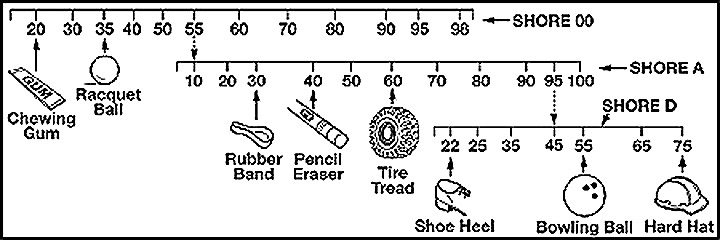
\includegraphics[width=0.85\textwidth]{imgs/shore_hardness.jpeg}
 	\caption{Shore Hardness scales, with some examples}
 \end{figure}
 
 \index{hardness!shore and durometer scales}
 \textit{Shore} or \textit{durometer} scales are suited to measuring elastomers (i.e. rubber). Again it is important to note there are different scales. 90A is much softer than 90D durometer. Material rated as 95A may be quite different than 45D, although they look like they are the same on the above chart. Colorants are often added to elastomers to make distinguishing between different hardnesses by eye easy.
 
 Elastomers are much harder to measure in other ways, and are often given ratings only by their durometer. While this is technically only a measure of hardness, it correlates reasonably well to other material properties like overall stiffness (harder being stiffer) and grip (softer being more interactive, or frictional).
 
 \subsection{Thermal Properties}
 \index{thermal characteristics}
 The thermal properties of a material may also be important to your application. There are three main ones to keep in mind if you are dealing with heat:
 \begin{asparaitem}
 	\item \textit{Thermal conductivity} is how well the material transfers heat. If you're designing a heat sink, you want a high thermal conductivity.
 	\item The \textit{melting point} or \textit{glass transition temperature} are temperatures at which the material undergoes fundamental phase changes. You obviously need to make sure your part doesn't outright melt, but you should also have a bit of margin, as the phenomenon called \textit{creep} can cause parts that are at elevated temperatures to deform over time, even though below melting point.
 	\item The \textit{coefficient of thermal expansion} measures how much material expands as it heats up. If you're working with tight-tolerance equipment (or extreme temperatures), you may need to keep an eye on this.
 \end{asparaitem}
  
\subsection{Other Properties} 
 
 Frictional characteristics and chemical interactions are very complex, and if you care about these, it will require some research beyond mere datasheets.
 
 Density is another property to be mindful of. Most properties given do not take this into account, and this is why many engineers may speak of a \textit{strength-to-weight ratio}. This is simply dividing the material property in question by the density of the material. This is a sensible comparison in many cases where weight is a concern. If we wanted to create a component to bear a certain load, we could use a material that was very strong but heavy, or use more of a lighter, but weaker material.
 
 \subsection{Material Comparisons}
 
 To actually get data to make material comparisons:
 \begin{asparaitem}
 	\item \href{http://www.matweb.com/search/DataSheet.aspx?MatGUID=3a2e111b27ef4e5d813bad6044b3f318&ckck=1}{\color{red}\underline{MatWeb}} has a wide range of material properties.
 	\item \href{https://www.makeitfrom.com/}{\color{red}\underline{MakeItFrom}} has a similarly wide range of materials, and includes a comparison tool to help evaluate different options.
 \end{asparaitem}
 
 Table \ref{table:materials} lists some common engineering materials' properties.
 
\begin{table}[H]
\begin{tabular}{rrrrrrr} 
\multicolumn{1}{c}{\textbf{Material}}                                                   & \multicolumn{1}{c}{\textbf{\begin{tabular}[c]{@{}c@{}}Density\\ {[}g/cm\textasciicircum{}3{]}\end{tabular}}} & \multicolumn{1}{c}{\textbf{\begin{tabular}[c]{@{}c@{}}Elastic\\ Mod. {[}GPa{]}\end{tabular}}} & \multicolumn{1}{c}{\textbf{\begin{tabular}[c]{@{}c@{}}Yield\\ {[}MPa{]}\end{tabular}}} & \multicolumn{1}{c}{\textbf{\begin{tabular}[c]{@{}c@{}}UTS\\ {[}MPa{]}\end{tabular}}} & \multicolumn{1}{c}{\textbf{\begin{tabular}[c]{@{}c@{}}\% Elong.\\ at Break\end{tabular}}} & \multicolumn{1}{c}{\textbf{\begin{tabular}[c]{@{}c@{}}Max Mech.\\ Temp {[}C{]}\end{tabular}}} \\ \hline
Aluminum 6061-T6                                                               & 2.7                                                                                                          & 69                                                                                            & 270                                                                                    & 310                                                                                  & 10                                                                                        & 170                                                                                           \\
Aluminum 7075-T6                                                               & 3.0                                                                                                          & 70                                                                                            & 480                                                                                    & 560                                                                                  & 8                                                                                       & 200                                                                                           \\
Steel, 4130-N                                                                  & 7.8                                                                                                          & 190                                                                                           & 440                                                                                    & 670                                                                                  & 26                                                                                        & 420                                                                                           \\
Steel, 4340-N                                                                  & 7.8                                                                                                          & 190                                                                                           & 860                                                                                    & 1280                                                                                 & 12                                                                                        & 420                                                                                           \\
Steel, 1020, Hot Rolled                                                        & 7.9                                                                                                          & 190                                                                                           & 240                                                                                    & 420                                                                                  & 28                                                                                        & 420                                                                                           \\
\begin{tabular}[c]{@{}r@{}}Stainless Steel,\\ 304, Annealed\end{tabular}      & 7.8                                                                                                          & 200                                                                                           & 230                                                                                    & 580                                                                                  & 43                                                                                        & 710                                                                                           \\
\begin{tabular}[c]{@{}r@{}}Titanium Grade 23\\ (Transformed-Beta)\end{tabular} & 4.4                                                                                                          & 110                                                                                           & 870                                                                                    & 930                                                                                  & 6.7                                                                                       & 340                                                                                           \\ \hline
Polycarbonate (PC) & 1.2                                                                                                          & 2.3                                                                                           & 62                                                                                     & 66                                                                                   & 110                                                                                       & 120                                                                                           \\
Acetal (Copolymer)                                                               & 1.4                                                                                                          & 2.8                                                                                           & *                                                                                      & 61                                                                                   & 65                                                                                        & 100                                                                                           \\
ABS                                                                            & 1.1                                                                                                          & 2.0                                                                                           & *                                                                                      & 41                                                                                   & 20                                                                                        & 80                                                                                            \\
PETG                                                                           & 1.3                                                                                                          & 2.2                                                                                           & *                                                                                      & 53                                                                                   & **                                                                                        & 70                                                                                            \\
Nylon 11                                                                       & 1.0                                                                                                          & 1.3                                                                                           & *                                                                                      & 51                                                                                   & 130                                                                                       & 180                                                                                           \\
\begin{tabular}[c]{@{}r@{}}Polypropylene (PP)\\ (Homopolymer)\end{tabular}      & 0.9                                                                                                          & 1.4                                                                                           & *                                                                                      & 36                                                                                   & 80                                                                                        & 120                                                                                           \\
PLA                                                                            & 1.3                                                                                                          & 3.5                                                                                           & *                                                                                      & 50                                                                                   & 6                                                                                         & 50                                                                                            \\
Acrylic                                                                        & 1.2                                                                                                          & 3.2                                                                                           & *                                                                                      & 71                                                                                   & 4                                                                                           & 100                                                                                          
\end{tabular}
* Plastics have odd stress-strain curves, so often don't rate the yield point. \\
** Extremely ductile; no data available
\caption{Common materials and their properties. Values obtained from MakeItFrom.com.}
 \label{table:materials}
\end{table}

A few interesting things to note:
\begin{asparaenum}[a)]
	\item Aluminum can be as strong as steel, not even considering the difference in density. The grade of steel and aluminum you're using is very important when comparing the two.
	\item Titanium is a truly incredible material. It is not quite as light as aluminum, but it is as strong as many high grades of steel!
	\item Among most metals, the \textit{stiffness-to-weight ratio} is about the same. If you want something to be stiffer without adding weight, only changing the type of metal won't help you out much.
	\item Plastics are much weaker, but they can be quite useful due to their low density: simply use more.
	\item Not all plastic is created equal.
	\item Polycarbonate and Nylon are particularly good materials for their mechanical properties, especially in impact resistance. Their elongation at break is \textbf{more than 100\%}!
\end{asparaenum}

 \section{Form Factors}
 
 Just because the material you want exists doesn't mean that it's widely available in the shape you want. There are a lot of different shapes that a material may be available in, and there are trade-offs with each different form factor.
 
 \subsection{Cast from Ingot}
\begin{figure}[H]
	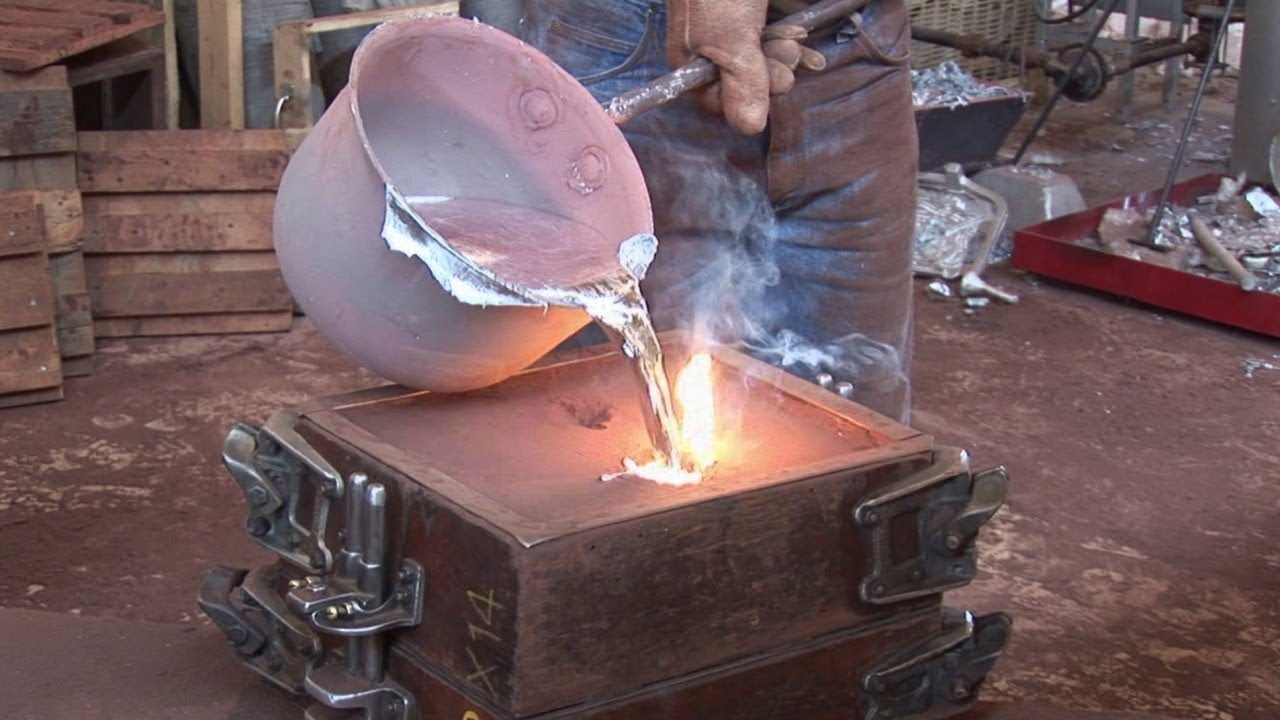
\includegraphics[width=0.55\textwidth]{imgs/casting_proc.jpeg}
	\qquad
	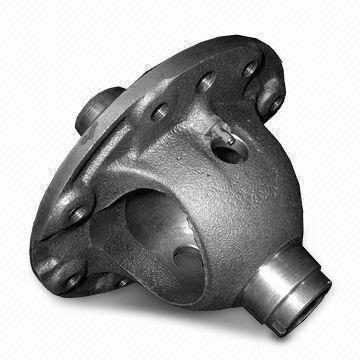
\includegraphics[width=0.3\textwidth]{imgs/casting_part.jpeg}
	\caption{Left: the casting process. Right: A cast differential housing.}
\end{figure} 
 \textit{Casting}\index{casting} is the process of pouring molten material into a mold to produce a complex shape. This shape isn't perfect, as the mold is usually made of sand (in order to withstand the molten metal) and the pouring process can introduce voids and imperfections, so the material properties are usually not as good. Cast parts have notably inferior material properties from billet or forged counterparts.
 
 \subsection{Billet and Plate}
 
 \begin{figure}[H]
	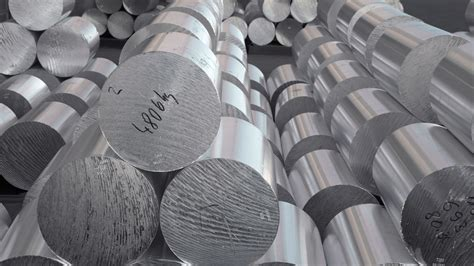
\includegraphics[width=0.6\textwidth]{imgs/billet.jpeg}
	\caption{Pieces of round billet.}
\end{figure} 
 \textit{Billet}\index{billet} material has been poured in a more tightly controlled environment. The resulting material is free of voids and has superior mechanical properties. You can obtain billet plate, bars, or round stock of nearly any material. This material can be held to reasonable tolerances (and by its simple-shaped nature, can be brought into exact dimension by machining quite easily).
 
 \subsection{Extrusions} \label{subsec:extrusions}
 \textit{Extruded}\index{extrusions} material has been squeezed through a die while molten, and then cooled. Think of a pasta machine. This die can be anywhere from a simple shape like a flat bar, to box tubing, to a very complicated profile with t-slots such as 80/20. Aluminum is the most common material to be extruded. Extrusions have good material properties, and can be held to tight tolerances.
 
  \begin{figure}[H]
	\begin{subfigure}[b]{.19\linewidth}
		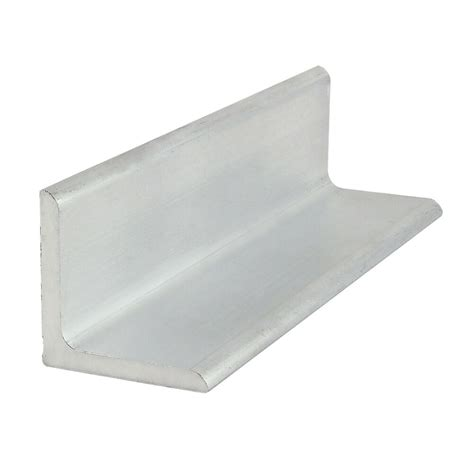
\includegraphics[width=0.95\textwidth]{imgs/extrusion_angle.jpeg}
		\caption{Angles}
	\end{subfigure} \begin{subfigure}[b]{.19\linewidth}
		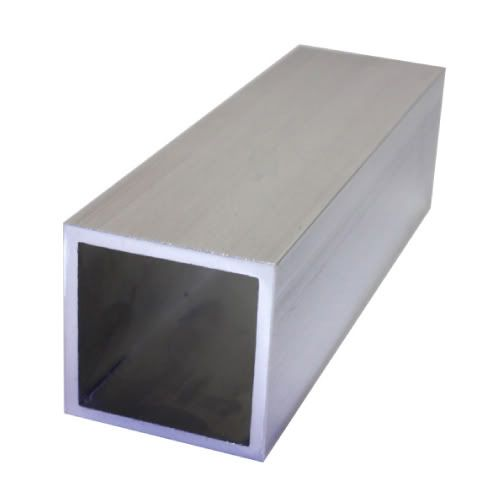
\includegraphics[width=0.95\textwidth]{imgs/extrusion_boxtube.jpeg}
		\caption{Box tube}
	\end{subfigure} \begin{subfigure}[b]{.19\linewidth}
		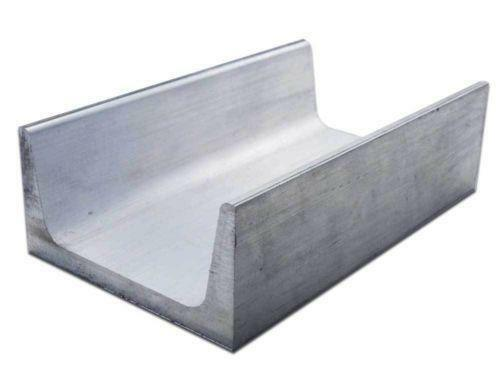
\includegraphics[width=0.95\textwidth]{imgs/extrusion_channel.jpeg}
		\caption{Box tube}
	\end{subfigure} \begin{subfigure}[b]{.19\linewidth}
		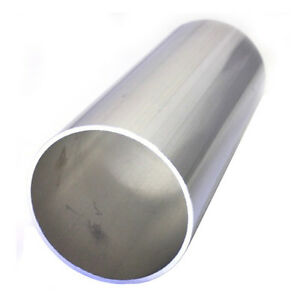
\includegraphics[width=0.95\textwidth]{imgs/extrusion_roundtube.jpeg}
		\caption{Pipe and tube}
	\end{subfigure}	\begin{subfigure}[b]{.19\linewidth}
		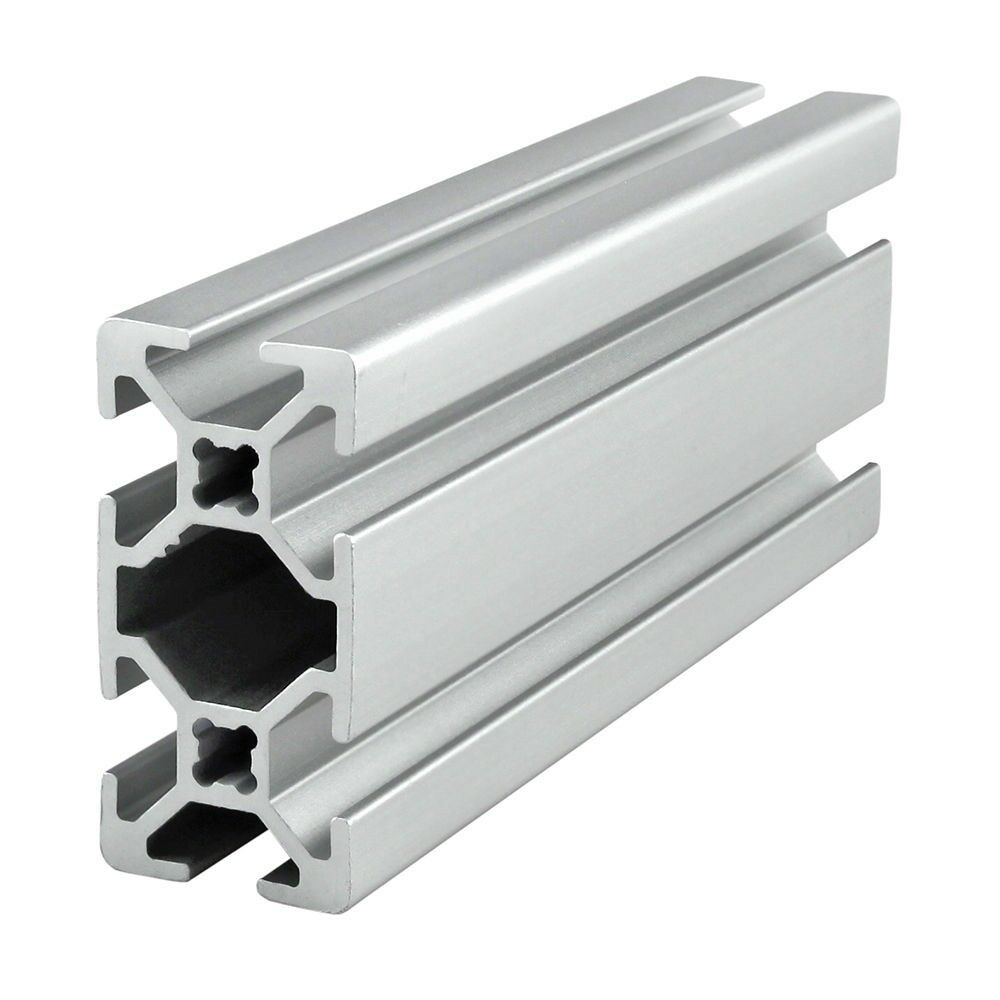
\includegraphics[width=0.95\textwidth]{imgs/extrusion_8020.jpeg}
		\caption{T-slot framing}
	\end{subfigure}	
	\caption{Common Extrusions}
\end{figure}

 \begin{asparaenum}[a)]
 	\item \textit{Angles} are measured by the leg width and the thickness. Only one dimension for leg lengths may be given if the leg lengths are equal. There may or may not be a radius in the corner, and radiuses on the tips of the legs.
 	\item \textit{Box tube} is measured by the outer side lengths and the thickness. It may or may not have an inner or outer radius - if it isn't specified, it probably doesn't.
 	\item \textit{Channel} is measured by the outer side lengths and the thickness. Usually it has straight walls of equal thickness, but it may have tapered, unequally sized walls.
 	\item \textit{Pipe and tube}\index{tube} is measured either by diameter and thickness, or by nominal pipe size and schedule. `1 inch' tube might refer to 1" nominal pipe, which actually has an inner diameter of 1.049", or a piece of tube with a 1" outer diameter. Make sure you know which you're buying.
 	\item \textit{T-slot framing}\index{extrusions!t-slot framing}, known often by the brand name \textit{80/20}, has several slots on the outside which t-slot nuts can be slid into. This makes creating configurable/adjustable frames easy, although the framing is quite heavy. 
 \end{asparaenum}
 
 \subsection{Welded / DOM Tubing} \index{tube}
 Steel is not easily extruded, so making hollow shapes must be tackled differently. Steel tubes are usually formed by taking sheet steel and rolling it into a tube, then welding it together. This process leaves a weld seam which can produce odd material properties, dimensional issues (as when making telescoping tubes), or make manufacturing annoying, as the weld is difficult to drill through). 
 
   \begin{figure}[H]
	\centering
	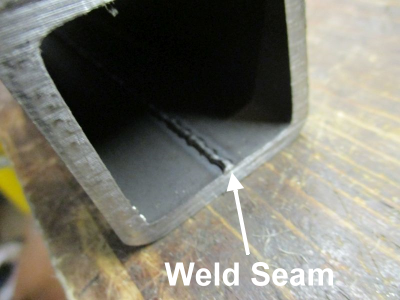
\includegraphics[width=0.4\textwidth]{imgs/welded_tube_seam.png}
	
	\caption{Weld Seam on Tubing}
\end{figure}
 
 \textit{DOM (Drawn-Over-Mandrel)} or \textit{seamless} tubing further processes this tubing to remove the inner seam and produce a product as if it were extruded. It is typically used in demanding applications such as aerospace or motorsports, as well as in components which cannot have a weld seam (such as a receiver hitch, or telescoping tubes).
 
 \subsection{Sheet}
 Material that is sold as sheet rather than plate usually has little-to-no straightness tolerance (in especially thin gauges, it might even be sold as rolls).
 
 \section{Manufacturing Processes}
 
 Once you have a material you like in a shape you can use, you probably have to cut or form it into the final shape you want. There are nearly infinite ways of doing this, but here are the most common.
 
 \subsection{Hot Work}
 
 Casting, sintering, and forging are manufacturing methods which generally require a lot of tooling in order to accomplish, so are generally not suitable for quick-turnaround prototypes such as we need. Some notes, though:
 
 \begin{asparaitem}
 	\item \textit{Casting}\index{casting} as mentioned before, is pouring molten metal into a mold. It can produce very complex shapes (like engine blocks), but the material may end up with lots of voids.
 	\item \textit{Forging}\index{forging} is heating up a metal so that it can be more easily formed, though not liquid. It is then pressed between large dies to form it into the desired shape- essentially, industrialized blacksmithing. Forging can produce fairly complex shapes (like crankshafts), while preserving (and even enhancing) material properties.
 	\item \textit{Sintering}\index{sintering} is compressing and heating powder in a mold. Also known as \textit{powder metallurgy}. This can produce somewhat simple parts with good material properties and no draft - many small gears are made this way.
 \end{asparaitem}
 
 \subsection{Machining}
 \index{machining!milling, drilling, and turning}
 Machining is a broad category of processes that cut material away with a sharp tool. There are many tools that can be used to accomplish this, but there are three that are the most essential and common:
 
 \begin{figure}[H]
	\centering
	\begin{subfigure}[b]{.24\linewidth}
		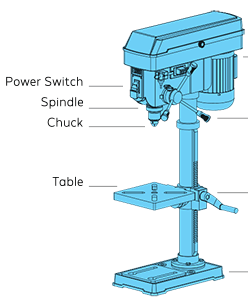
\includegraphics[width=0.95\textwidth]{imgs/drillpress.png}
		\caption{Drill press}
	\end{subfigure}	\begin{subfigure}[b]{.34\linewidth}
		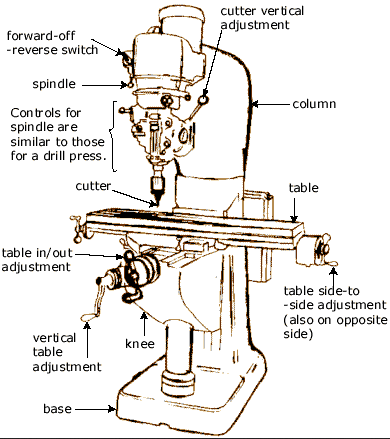
\includegraphics[width=0.95\textwidth]{imgs/mill.png}
		\caption{Milling machine}
	\end{subfigure}	\begin{subfigure}[b]{.4\linewidth}
		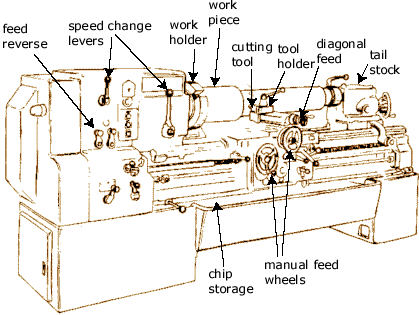
\includegraphics[width=0.95\textwidth]{imgs/lathe.png}
		\caption{Lathe}
	\end{subfigure}	
	
	\caption{The Most Common Machining Tools}
\end{figure}

 \begin{asparaenum}[a)]
 	\item A \textit{drill press}\index{drill press} has a rotating spindle and chuck where drillbits can be inserted. Workpieces are clamped to a fixed table. The spindle can then be brought down and into the work to drill holes.
 	\item A \textit{milling machine}\index{milling machine} has a rotating spindle where drill bits and mill bits - end mills - can be inserted. Workpieces are secured to a table that moves along X, Y, and Z axes with respect to the spindle. \textit{Routers} operate by the same principle, but generally refer to a tool which moves much more in the X and Y than the Z, and may not be as rigid; more suitable to cutting sheets of plywood or foam.
 	\item A \textit{lathe}\index{lathe} has a rotating spindle in which the workpiece is held securely. Cutting tools are mounted to a carriage which moves axially and radially, shaping the exterior of the work. Additionally, a tailstock can accept drill bits and other supporting devices.
 \end{asparaenum}
 
  There are lots of variations on these machines: combinations of these exist, and 4- and 5- axis mills where the head or table tilt on the fly also exist. They can also all be enhanced with the addition of \textit{CNC}\index{CNC} (Computerized Numeric Control) in order to produce even more complicated shapes and/or increase productivity.
  
 These different machines can accept a wide variety of cutting implements. Here are a few of the most common to consider.
 
 \begin{figure}[H]
	\begin{subfigure}[b]{.19\linewidth}
		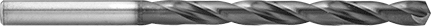
\includegraphics[width=0.95\textwidth,angle=-17]{imgs/drillbit.png}
		\caption{Drillbit}
	\end{subfigure} \begin{subfigure}[b]{.19\linewidth}
		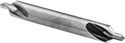
\includegraphics[width=0.95\textwidth]{imgs/centerdrill.png}
		\caption{Center drill}
	\end{subfigure} \begin{subfigure}[b]{.19\linewidth}
		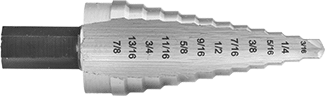
\includegraphics[width=0.9\textwidth,angle=-17]{imgs/step_drill.png}
		\caption{Step drill}
	\end{subfigure}\begin{subfigure}[b]{.19\linewidth}
		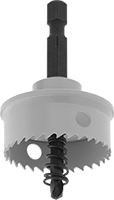
\includegraphics[width=0.45\textwidth,angle=73]{imgs/hole_saw.png}
		\caption{Hole Saw}
	\end{subfigure}\begin{subfigure}[b]{.19\linewidth}
		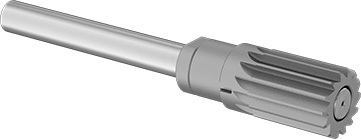
\includegraphics[width=0.95\textwidth]{imgs/reamer.png}
		\caption{Reamer}
	\end{subfigure}
	\caption{Holemaking tools}
\end{figure}

 \begin{asparaenum}[a)]
 	\item \textit{Drill bits} drill holes. The spiral flutes on the outside may be sharp, but they generally aren't sharp or hard enough to actually cut metal. They work with Jacobs chucks, which are designed to only transmit vertical force and torque.
 	\item \textit{Center drills} are used to start holes. They are short and stubby, so don't deflect much.
 	\item \textit{Step drills} have multiple steps in them that can be used to quickly make large holes. These can sometimes produce holes with good tolerances for slip-fits on bearings ($\approx \pm$ 0.005").
 	\item \textit{Hole saws} are effective at quickly removing large disks of materials. Typical bi-metal hole saws are not very precise, but well constructed carbide-tipped hole saws can achieve tight tolerances ($\approx \pm$ 0.002").
 	\item \textit{Reamers} enlarge existing holes to precise ($\approx \pm$ 0.0002") diameters. They are used by first drilling a hole about 1/32" smaller than the target diameter and then running the reamer in.
 \end{asparaenum}

\begin{figure}[H]
	\begin{subfigure}[b]{.19\linewidth}
		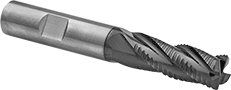
\includegraphics[width=0.95\textwidth]{imgs/endmill.png}
		\caption{End mill}
	\end{subfigure}	\begin{subfigure}[b]{.19\linewidth}
		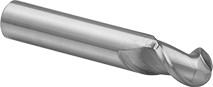
\includegraphics[width=0.95\textwidth]{imgs/ball_endmill.png}
		\caption{Ball end mill}
	\end{subfigure}\begin{subfigure}[b]{.19\linewidth}
		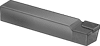
\includegraphics[width=0.95\textwidth]{imgs/lathetool.png}
		\caption{Lathe tooling}
	\end{subfigure}	
	
	\caption{Machine Tooling}
\end{figure}

\index{machining!tooling}
\begin{asparaenum}[a)]
 	\item \textit{End mills} cut on all surfaces - they are all ground sharp. This means they can cut on the side, and produce side loads - so they should not be put in Jacobs chucks in drill presses!
 	\item \textit{Ball end mills} are an example of a more sophisticated end mill. There are many different shapes. This one enables smooth contours to be made.
 	\item \textit{Lathe tooling} comes in many different shapes and sizes. This one is a simple cutting tool that gets clamped to the toolpost and shapes the outside of the work.
 \end{asparaenum}
 
If you can consider briefly how these machines work, you can perhaps spot a few problems with your designs as you go along. Can you spot some issues with these parts?
 
\begin{figure}[H]
	\centering
	\begin{subfigure}[b]{.24\linewidth}
		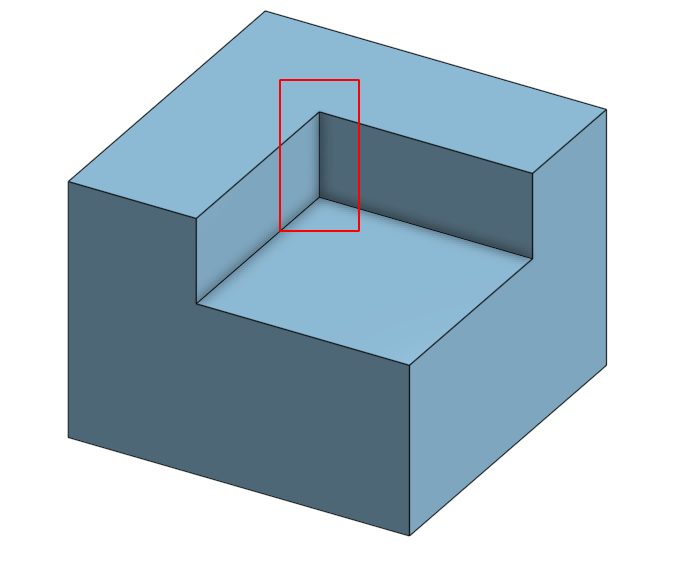
\includegraphics[width=0.9\textwidth]{imgs/nonmill_sharpins.png}
		\caption{Sharp inside corner}
	\end{subfigure}	\begin{subfigure}[b]{.24\linewidth}
		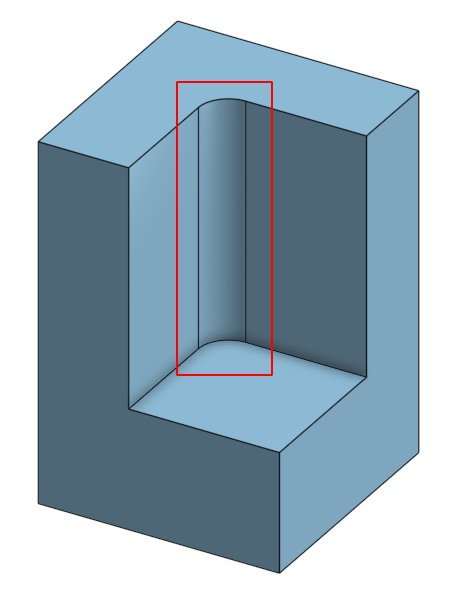
\includegraphics[width=0.9\textwidth]{imgs/nonmill_dtod.png}
		\caption{Deep radius}
	\end{subfigure}	
	
	\caption{Problematic geometries for machining}
\end{figure}

 \begin{asparaenum}[a)]
 	\item The sharp inside corner cannot be made, as it would require an infinitely small diameter tool.
 	\item The deep radius would require a very long end mill, which would not be very stiff. This radius is 0.25", and it is 2" tall; this is a ratio of depth-to-diameter of 4:1, which is a sub-optimal ratio. Ideally, this ratio would be no more than 3:1.
 \end{asparaenum}
 
 \subsection{Broaching}
 
 
 \begin{figure}[H]
 	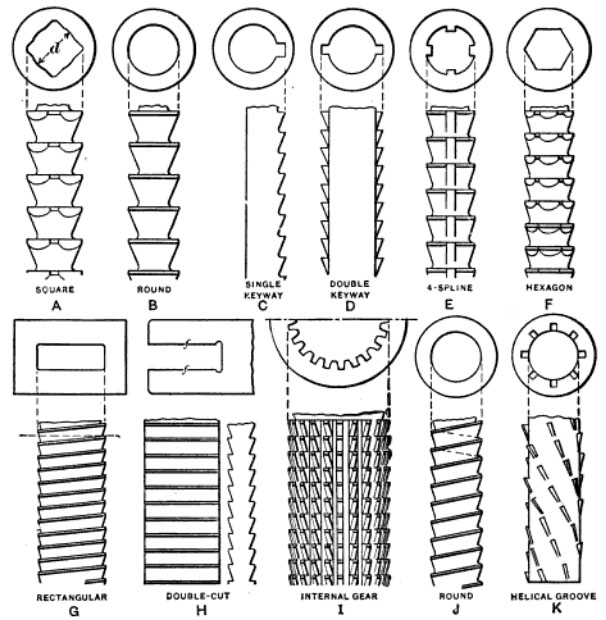
\includegraphics[width=0.6\textwidth]{imgs/broach_examples.jpeg}
 	\caption{Broach Examples}
 \end{figure}
 
 But how do we make splines, keyways, and hexes in things? Those need infinitely sharp corners, so we broach them. This is done by first drilling a hole of the appropriate diameter, and then inserting a broaching tool into the hole. The tool is then pushed through with a press. Each tooth of the broach takes off gradually more material until the final shape is achieved. Broaches are typically very expensive and relatively delicate tools.
 
 \begin{figure}[H]
 	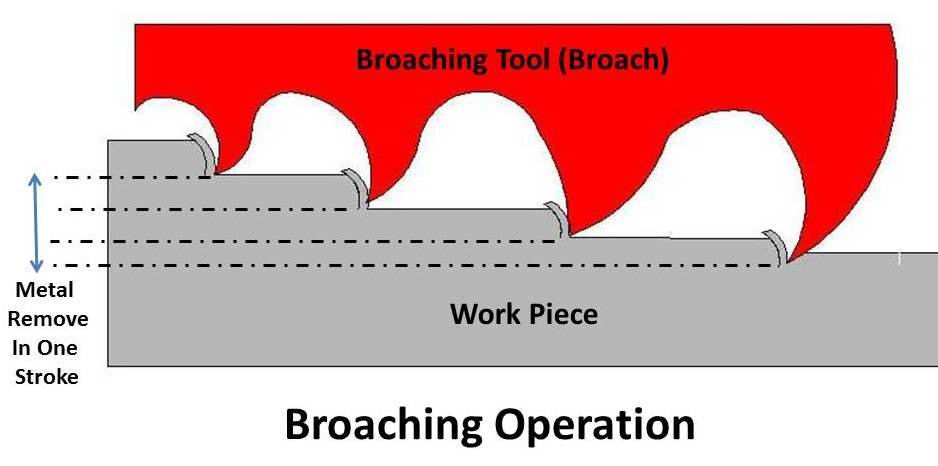
\includegraphics[width=0.7\textwidth]{imgs/broach_detail.jpeg}
 	\caption{Broach Detail}
 \end{figure}
 
 
 \subsection{Path Cutting}
 
 \textit{Path cutting}\index{path cutting} is encompasses any sort of 2-dimensional X/Y cutting with a thin beam. It is almost always done on a CNC-capable machine.
 
 \begin{figure}[H]
		\begin{subfigure}[b]{.24\linewidth}
			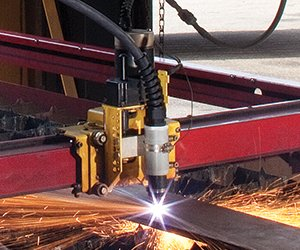
\includegraphics[width=0.9\textwidth]{imgs/plasmacut.jpeg}
			\caption{Plasma cutting}
		\end{subfigure}\begin{subfigure}[b]{.24\linewidth}
			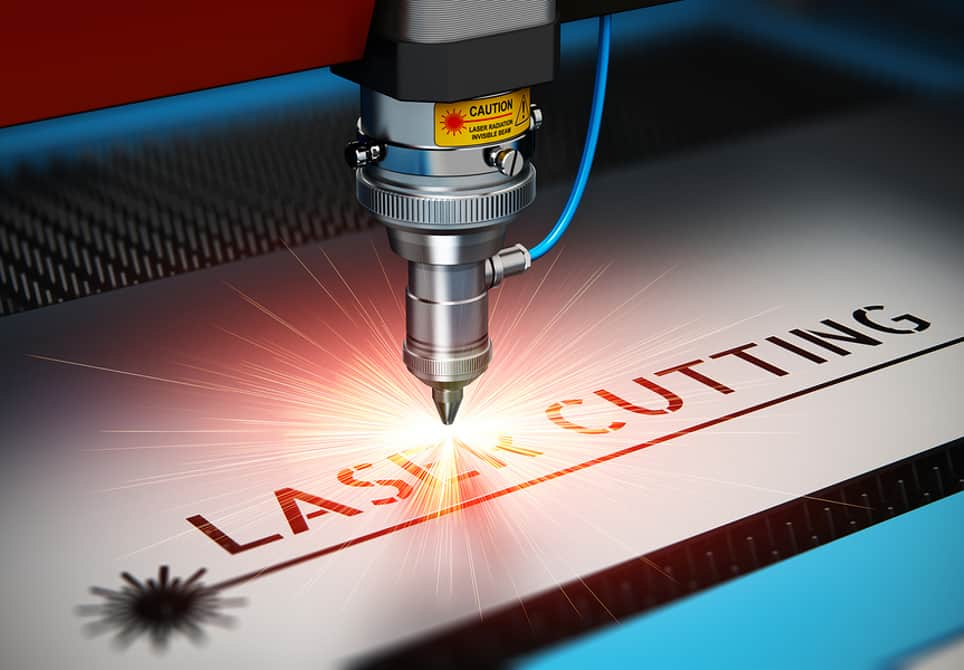
\includegraphics[width=0.9\textwidth]{imgs/lasercut.jpeg}
			\caption{Laser cutting}
		\end{subfigure}\begin{subfigure}[b]{.24\linewidth}
			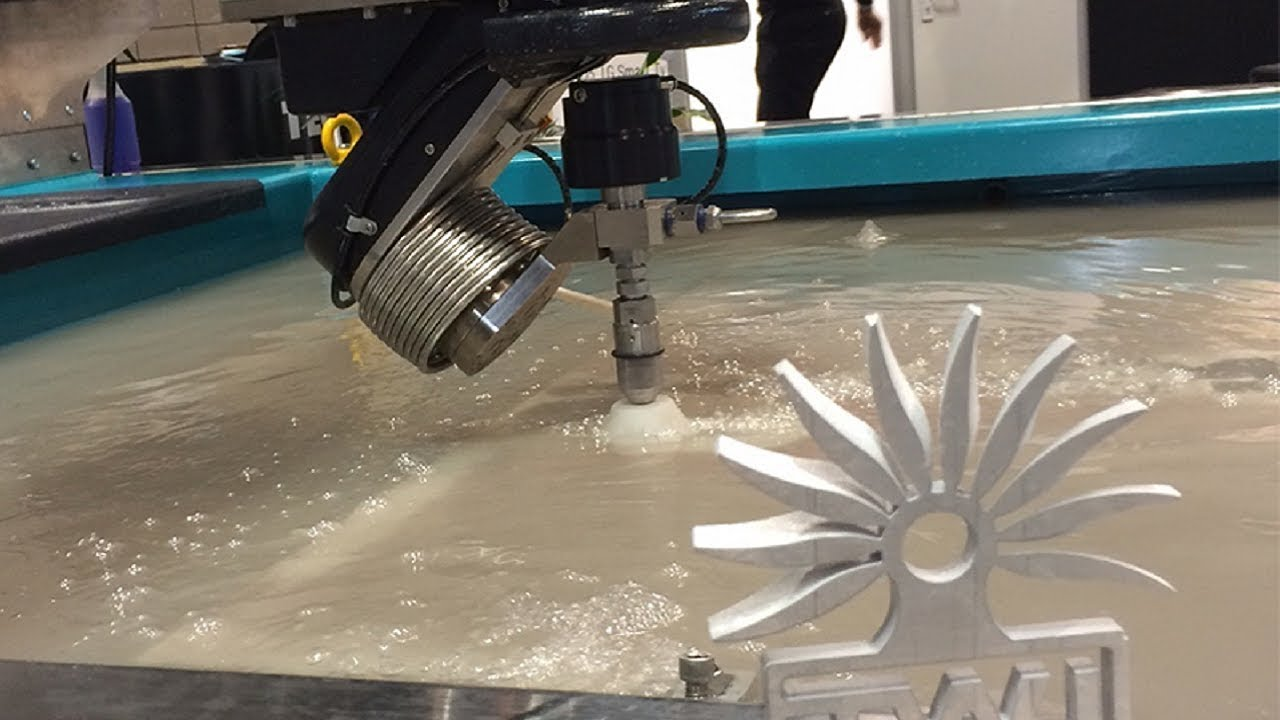
\includegraphics[width=0.9\textwidth]{imgs/waterjet.jpeg}
			\caption{Waterjet cutting}
		\end{subfigure}\begin{subfigure}[b]{.24\linewidth}
			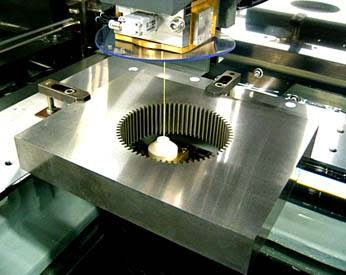
\includegraphics[width=0.9\textwidth]{imgs/edm.jpeg}
			\caption{EDM cutting}
		\end{subfigure}
	\end{figure}
 
 \begin{asparaenum}[a)]
  	\item \textit{Plasma cutters}\index{path cutting!plasma cutting} use an arc to melt metal and pressurized air to blow it away. The tolerances are usually good for large shapes, but not for precision work.
 	\item \textit{Laser cutters}\index{path cutting!laser cutting} melt material with a laser and either simply vaporize it or use pressurized air to blow it away. Hobby lasers can cut some plastics and plywood, while industrial systems can cut metal. The tolerances are usually acceptable with these machines ($\pm 0.020"$).
 	\item \textit{Waterjet cutters}\index{path cutting!waterjet cutting} mix high-pressure water with garnet sand and blast it at material, rapidly abrading it. The tolerances are usually good with this process ($\pm 0.010"$ or better).
 	\item \textit{EDMs}\index{path cutting!EDM} (electric-discharge-machines) use an electrified wire to remove material. The wire is fed through or plunged into material. The electrification zaps away material next to the wire. The tolerances with this process can be impeccable ($\pm 0.001"$ or better). 
\end{asparaenum}
 	
 	These all allow us to overcome the depth-to-diamter ratio imposed by milling, and can sometimes be much quicker setup than traditional machining, though they all come with their own drawbacks.
 
 \begin{figure}[H] \centering
 	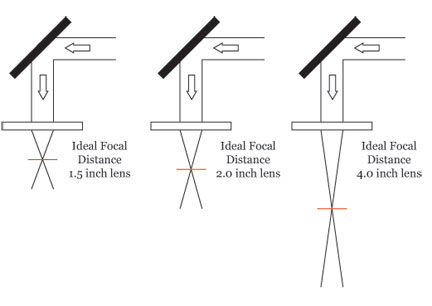
\includegraphics[width=0.5\textwidth]{imgs/lasercut_focus.jpeg}
 	\caption{Focal properties of a laser cutter's beam.}
 \end{figure}
 
  The first limitation is the width of the beam. Since a finitely sized beam muse be used, infinitely sharp interior corners cannot be made.
 
 \begin{figure}[H] \centering
 	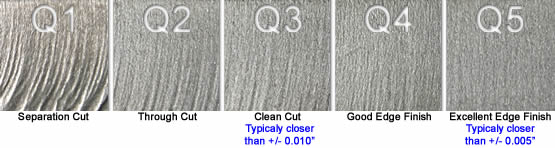
\includegraphics[width=0.9\textwidth]{imgs/waterjet_draft.jpeg}
 	\caption{Draft and surface quality samples on a waterjet with different settings.}
 \end{figure}
 
  The next consideration that must be made is draft. Laser-cutters typically have a point in the thickness where the beam is focused to. This means that the laser doesn't cut a line in its cross-section, but rather an X. Thus the resulting shape is two-dimensional. With a waterjet or plasma cutter, the draft grows exponentially. This may be acceptable, or require further post-machining to bring it into specification.
 
 Draft (and power) also limits how thick of material can feasibly be cut with these processes, although it should be noted that EDM can cut extremely thick materials compared to the other processes.
 
 \subsection{Sheet Forming}
 \index{sheet metal!forming}
 \index{sheet metal!bending}
 Sheet forming is a versatile process of making parts from, well, sheet. Sheet may be cut with either a stamping or path-cutting operation to form a blank. This blank can then be loaded in and undergo one of several processes.
 
 	\begin{figure}[H]
		\centering
		\begin{subfigure}[b]{.24\linewidth}
			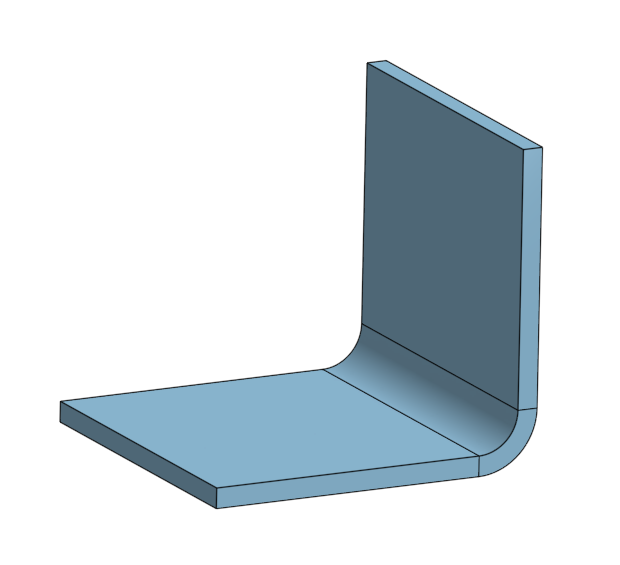
\includegraphics[width=0.9\textwidth]{imgs/sheet_bend.png}
			\caption{Bend}
		\end{subfigure}\begin{subfigure}[b]{.24\linewidth}
			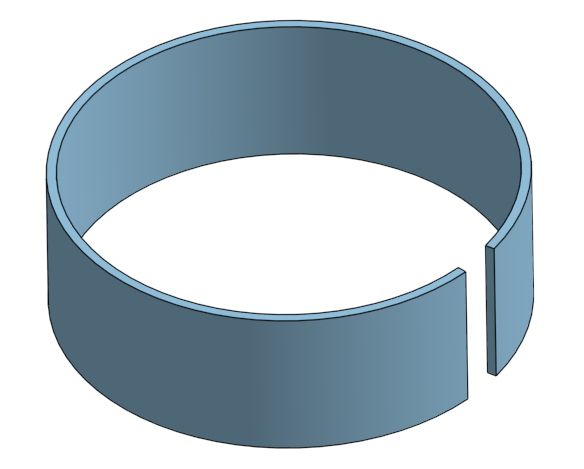
\includegraphics[width=0.9\textwidth]{imgs/sheet_roll.png}
			\caption{Rolling}
		\end{subfigure}\begin{subfigure}[b]{.24\linewidth}
			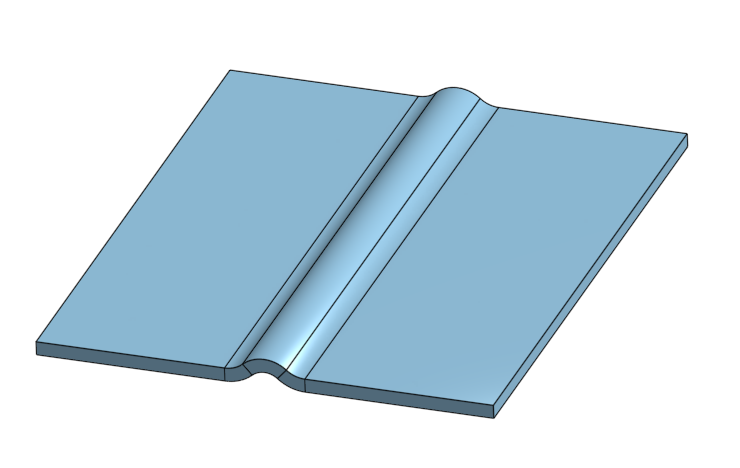
\includegraphics[width=0.9\textwidth]{imgs/sheet_beadroll.png}
			\caption{Bead Rolling}
		\end{subfigure}\begin{subfigure}[b]{.24\linewidth}
			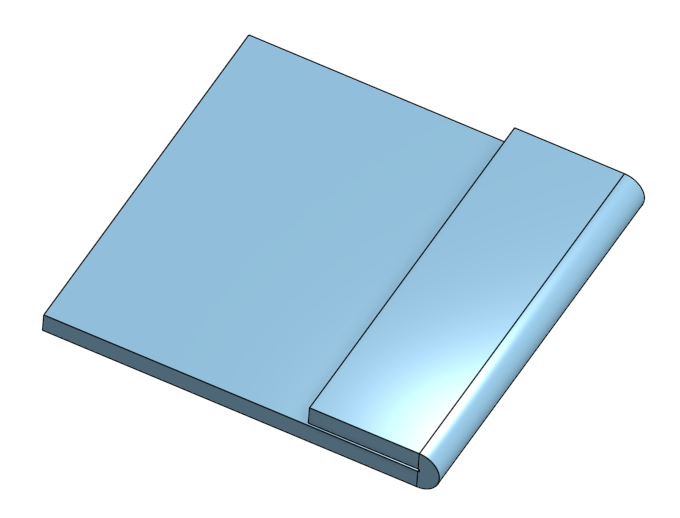
\includegraphics[width=0.9\textwidth]{imgs/sheet_hem.png}
			\caption{Hemming}
		\end{subfigure}
		\caption{Rudimentary sheetmetal operations.}
	\end{figure} 
 
 \begin{asparaenum}[a)]
 	\item Simple \textit{bends} can be made on a linear portion of the flat pattern. This can be done with a finger bender, press brake, or, in a pinch, a vise with a hammer.
 	\item Flat portions of material can be \textit{rolled} into an arc, or even full circle.
 	\item \textit{Bead rolling} can be done on any portion of a part to provide additional stiffness.	
 	\item \textit{Hemming} provides a smooth, radiused outer corner and some additional stiffness. First, a bend is made, and then it is bent all the way to 180 degrees. This can be done with a finger bender or press brake, and additional clamping to finish the hem.
 	\end{asparaenum}
 	
 	Most CAD packages have tools to design parts made with sheet metal. You can draw up the bent part, and then the CAD package will determine how to unfold and produce a flat pattern that can be cut out.
 	
 	These operations are typically done with metal, but nothing prevents them from being applied to plastic. Polycarbonate can be bent like sheet metal. Polypropylene, polycarbonate, acrylic, and PETG, among others, can be heated - heat gun or other method - and then bent by hand.
 	
 	\subsection{Welding and Brazing}
 	\index{welding!MIG, TIG, stick and arc}
 	Welding and brazing are very important manufacturing methods. They enable large, complex structures to be made from smaller simple ones without fasteners that might fail. However, it requires time consuming labor and creates non-serviceable structures.
 	
 	\begin{figure}[H]
		\centering
		\begin{subfigure}[b]{.24\linewidth}
			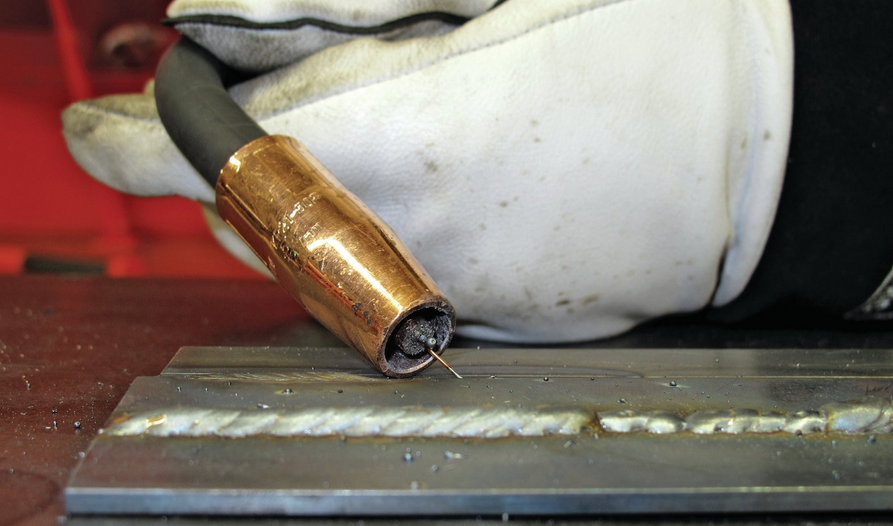
\includegraphics[width=0.9\textwidth]{imgs/mig.png}
			\caption{MIG}
		\end{subfigure}\begin{subfigure}[b]{.24\linewidth}
			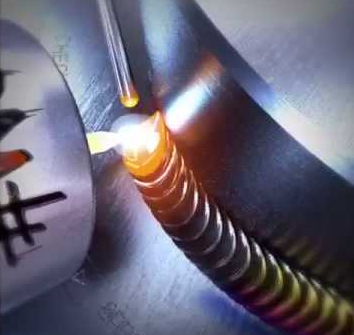
\includegraphics[width=0.9\textwidth]{imgs/tig.png}
			\caption{TIG}
		\end{subfigure}\begin{subfigure}[b]{.24\linewidth}
			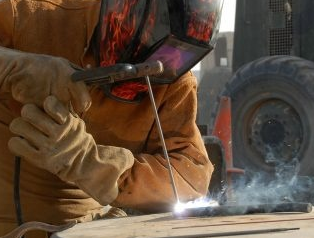
\includegraphics[width=0.9\textwidth]{imgs/arcweld.png}
			\caption{Stick/Arc Welding}
		\end{subfigure}\begin{subfigure}[b]{.24\linewidth}
			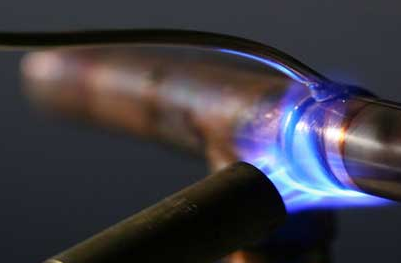
\includegraphics[width=0.9\textwidth]{imgs/braze.png}
			\caption{Brazing}
		\end{subfigure}
		\caption{Various welding/brazing technologies.}
	\end{figure}
 	
 	\begin{asparaenum}[a)]
 		\item \textit{MIG} (Metal-Inert-Gas) welding uses an electric arc between filler wire and the workpiece, which melts both the wire and the workpiece. The arc is shielded by inert or semi-active gas to control chemical reactions. The wire is advanced at a constant rate into the workpiece. This is the easiest method to learn, but provides the least amount of control, and has the lowest capacity for superior results.
 		
 		\item \textit{TIG} (Tungsten-Inert-Gas) welding uses an electric arc between a fixed tungsten rod and the workpiece, melting the work but not the tungsten. The arc is shielded by inert gas to eliminate chemical reactions. Filler rod is advanced manually and separately into the molten work. This method is much harder to learn, but provides the most amount of control, with the highest capacity for superior results.
 		
 		\item \textit{Stick/Arc} welding uses an electric arc between a rod containing flux and filler metal and the workpiece, melting both the rod and the workpiece. The arc is shielded by the vaporizing flux. This method is hard to learn, but provides good control, and works best outdoors, so is quite common in the construction and pipeline industries.
 		
 		\item In \textit{brazing}\index{brazing}, heat is generated either by a TIG or flame torch and directed at the work without melting it. Brazing material, which will melt at this surface temperature, is fed onto the work, melting and flowing across it. As it solidifies, it adheres to the base metal.
 		
 	\end{asparaenum}
 	
 	\subsection{3D Printing}
 	\index{3D printing}
 	\index{3D printing!additive manufacturing}
 	\textit{3D printing} or \textit{additive manufacturing} is a varied class of technologies that add material selectively and in a discretely controlled fashion. This allows the production of extremely complex geometries with little to no tooling costs, but is a pioneering field and has many limitations.
 	
 	\begin{figure}[H]
		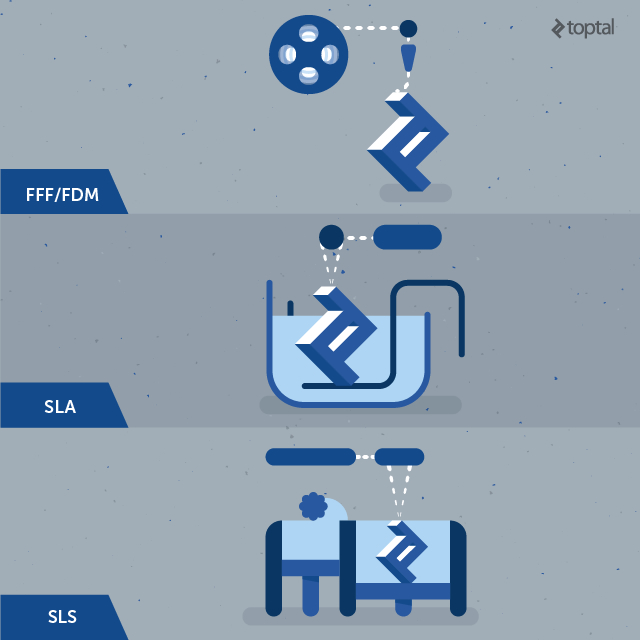
\includegraphics[width=0.9\textwidth]{imgs/3dp_fdm_sla_sls.jpeg}
		\caption{Major 3D printing technologies.}
	\end{figure}
 	
 	\begin{asparaenum}[a)]
 		\item \textit{Fused deposition modeling (FDM)}\index{3D printing!FDM} uses a continuous piece of plastic filament which is heated in the \textit{hot end} before being squeezed through an \textit{extruder} to lay down thin layers of material which melt into previous layers. This method is quite reliable and cheap, but does result in models with visible layers, and generally results in models where the strength can vary with the orientation of the layers.
 		Because it works by melting existing material, it is limited to materials that can be melted and cooled into final form such as thermoplastics. Common materials are PLA, ABS, and to an increasing extent, PETG, Polycarbonate, and Nylon. FDM is furthermore is limited in that it cannot print steep overhangs without wasteful or surface-quality changing \textit{support material}\index{3D printing!support}. Porosity and sealing can also be concerns. On the upside, it can create hollow parts, enabling high strength-to-weight ratios as material can be placed only where it is needed.
 		\textit{Continuous-strand reinforcement}\index{3D printing!continuous-strand reinforcement} is a new addition to this technology. As the name implies, this is the inclusion of a fibrous high-strength material such as fiberglass or carbon fiber into the filament, so that when it is extruded, the part has many strands of this reinforcing material. Markforged makes printers capable of this.
 		\item \textit{Stereolithography (SLA)}\index{3D printing!SLA} uses a laser to quickly cure liquid \textit{resin} into solid material. The print bed moves away from the laser as additional layers are added. This method is inherently limited to materials that can be made from resins, ruling out many materials. It is a quite time-consuming process but can result in parts with good sealing properties and excellent surface finish. Hollow parts cannot be created as the resin would simply be trapped inside cavities. Formlabs is a prominent manufacturer of such printers.
 		\item \textit{Selective laser sintering (SLS)}\index{3D printing!SLS} uses a laser to selectively melt and \textit{sinter} powdered material together. After one layer is sintered, another thin layer of powder is put over top, and the process repeats. This process can achieve excellent mechanical properties which are not dependent on layer orientation, as well as stellar dimensional accuracy. However, it results in parts with a very coarse surface texture. Hollow parts cannot be created as the powder would simply be trapped inside cavities. The continuous addition of powder (of which the unsintered material can be reused) allows for the production of parts with infinitely sharp overhangs since the previous layer acts as support material.
 	\end{asparaenum}
 	
 	Metal 3D printing technologies are also in the works, most being a modification of the traditional SLS method with metal powders.
 		
	\section{Fasteners}
	Fasteners are a broad family of mechanical solutions to fastening parts together.
	
	\subsection{Pins}
	\index{pins}	
	The simplest fastener is a pin. Pins prevent plate holes from shearing past each other by putting all of the load through the pin. There are a couple different kinds, each with different properties:
	
	Quick pins allow users to easily adjust or reconfigure equipment. They are easily insertable/removable, usually without any special tools.
	
	\begin{figure}[H]
		\centering
		\begin{subfigure}[b]{.32\linewidth}
			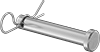
\includegraphics[width=0.7\textwidth]{imgs/cpin.png}
			\caption{Clevis pin}
		\end{subfigure}\begin{subfigure}[b]{.32\linewidth}
			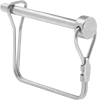
\includegraphics[width=0.7\textwidth]{imgs/wlpin.png}
			\caption{Wire-locking pin}
		\end{subfigure}\begin{subfigure}[b]{.32\linewidth}
			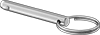
\includegraphics[width=0.7\textwidth]{imgs/bdpin.png}
			\caption{Ball-detent pin}
		\end{subfigure}
		\caption{Various quick-removal pins.}
	\end{figure}
	
	\begin{asparaenum}[a)]\index{pins!quick}
		\item \textit{Clevis pins} are loose tolerance pins which have a hole for an R-shaped locking pin or wire to go through.
		\item \textit{Wire-locking pins} serve the same purpose as clevis pins, but use a spring-loaded wire to keep the pin captive.
		\item \textit{Ball-detent pins} serve the same purpose as clevis pins, but use a spring-loaded ball detent to keep the pin captive. These can be pulled/pushed in without and additional steps.
	\end{asparaenum}
	
	
	Precision pins serve a nearly opposite purpose- they are permanent installations, but provide extremely tight tolerances when used right. They allow for installation and detachment of components with high repeatability in locational positioning. It's not uncommon to see precision equipment register together with pins, and then be bolted together in addition to the pins. Pins also can provide higher load transferral because they do not have the stress concentrators that bolts do.
	
	\begin{figure}[H]
		\centering
		\begin{subfigure}[b]{.19\linewidth}
			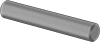
\includegraphics[width=0.85\textwidth]{imgs/dpin.png}
			\caption{Dowel pin}
		\end{subfigure}\begin{subfigure}[b]{.19\linewidth}
			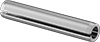
\includegraphics[width=0.85\textwidth]{imgs/spin.png}
			\caption{Spring pin}
		\end{subfigure}\begin{subfigure}[b]{.19\linewidth}
			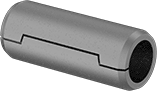
\includegraphics[width=0.7\textwidth]{imgs/hollow_dpin.png}
			\caption{Hollow dowel pin}
		\end{subfigure}\begin{subfigure}[b]{.19\linewidth}
			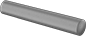
\includegraphics[width=0.85\textwidth]{imgs/tpin.png}
			\caption{Taper pin}
		\end{subfigure}\begin{subfigure}[b]{.19\linewidth}
			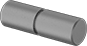
\includegraphics[width=0.75\textwidth]{imgs/shpin.png}
			\caption{Shear pin}
		\end{subfigure}
		\caption{Various precision pins.}
	\end{figure}
	
	\begin{asparaenum}[a)]
		\item \textit{Dowel pins}\index{pins!dowel} are tight-tolerance. They are typically pressed into one part's hole with a loose fit on another mating part.
		\item \textit{Spring pins} are formed from coiled metal and are intended to be pressed in like a dowel pin, but have some give to them so that they can be used with looser-tolerance holes.
		\item \textit{Hollow dowel pins} serve the same purpose as dowel pins but allow a bolt to pass through them as well. 
		\item \textit{Taper/scotch pins} are like dowel pins, but they are slightly tapered, so they wedge into multiple parts like a nail.
		\item \textit{Shear pins} are specifically designed to fail at a specified load, preventing damage to equipment.
	\end{asparaenum}
	
	\subsection{Threads} \label{subsec:threads}
	\index{thread}
	Threaded fasteners (bolts, nuts, and screws) are a ubiquitous solution. There's an age old question of the difference between a screw and a bolt and the answer is merely in application: if it goes into a nut, it's a bolt. Otherwise, it's a screw. So, anything said about screws is true of bolts and vice versa.
	
	\begin{figure}[H]
		\includesvg{dwgs/screw}
		\caption{Thread nomenclature and dimensions.}
	\end{figure}
	
	Threaded fasteners are denoted by:
	\begin{asparaitem}
		\item The major diameter of the thread.
		\item The thread \textit{pitch}\index{thread!pitch}, or threads-per-inch. Metric bolts are specified by the pitch (a M5x0.8 has 0.8mm between each thread crest). English bolts are specified by the number of thread crests in an inch (a 1/4"-20 has 20 threads per inch, or a pitch of 1/20 = 0.05 inches). Even among the same diameter, bolts can have different pitches. For instance, a 1/4"-28 is fine thread, and a 1/4"-20 is coarse thread.
		\item The thread length - the bolt might be threaded fully, or only partially. The unthreaded portion is the shoulder and is usually the same diameter as the threads' major diameter.
		\item The handedness of the thread - most threads are right handed (meaning turning them in a clockwise fashion will make them move away) unless specified as left-handed.
		\item The grade or class - this refers to the strength of the material. English bolts are specified by \textit{grade}\index{thread!grade}, and metric bolts by \textit{class}\index{thread!class}. Bolts usually have head markings that reflect the material. Grade and class are only for steel, though - other materials have more exotic standards.
	\end{asparaitem}
	
	There are many different types of bolts out there.
	\index{screws and bolts}
	\begin{figure}[H]
		\centering
		\begin{subfigure}[b]{.24\linewidth}
			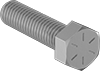
\includegraphics[width=0.7\textwidth]{imgs/hhcs.png}
			\caption{External drive}
		\end{subfigure}\begin{subfigure}[b]{.24\linewidth}
			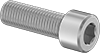
\includegraphics[width=0.7\textwidth]{imgs/shcs.png}
			\caption{Socket head}
		\end{subfigure}\begin{subfigure}[b]{.24\linewidth}
			\includegraphics[width=0.7\textwidth]{imgs/fhcs.png}
			\caption{Flathead}
		\end{subfigure}\begin{subfigure}[b]{.24\linewidth}
			\includegraphics[width=0.7\textwidth]{imgs/bhcs.png}
			\caption{Button head}
		\end{subfigure}
		
		\begin{subfigure}[b]{.24\linewidth}
			\includegraphics[width=0.7\textwidth]{imgs/shoulderscrew.png}
			\caption{Shoulder screw}
		\end{subfigure}\begin{subfigure}[b]{.24\linewidth}
			\includegraphics[width=0.7\textwidth]{imgs/stscrew.png}
			\caption{Self-tapping screw}
		\end{subfigure}\begin{subfigure}[b]{.24\linewidth}
			\includegraphics[width=0.7\textwidth]{imgs/carriagebolt.png}
			\caption{Carriage bolt}
		\end{subfigure}\begin{subfigure}[b]{.24\linewidth}
			\includegraphics[width=0.7\textwidth]{imgs/grubscrew.png}
			\caption{Grub or set screw}
		\end{subfigure}
		\caption{Various screws / bolts.}
	\end{figure}
	
	\index{screws and bolts!types}
	\begin{asparaenum}[a)]
		\item \textit{External drive} bolts are good when only side-access is possible. The most common example is a hex-head bolt, though pentagon-, external-torx-, and square- heads exist. They are usually the most resistant to stripping out. Versions with a flange at the base also exist to help distribut load and allow sockets to push on the screw.
		\item \textit{Socket head} bolts are preferred. They can be installed in deep wells and have a compact head profile.
		\item \textit{Flat head} screws need to be installed into holes that have been countersunk to the same angle as the head of the screw. They allow for a flush, smooth installation.
		\item \textit{Button head} screws provide a smooth surface without the need to countersink the surface.
		\item \textit{Shoulder screws} are special-use screws. The shoulder (unthreaded) portion is precision ground and usually a larger diameter than the thread. This allows them to be used as pins or pivot points.
		\item \textit{Self-tapping screws} have specially formed tips based on what material they are designed to tap into. They thread into material directly; a tap is not required to form threads, and in plastic and wood, are generally stronger.
		\item \textit{Carriage bolts} have a rounded head without any means of being driven externally. Instead, the square portion sitting under the thread mates with the material it bolts together (either a plate with the corresponding female portion, or a soft material like wood conforms to the square). \textit{Plow bolts} are the same principle, but are flat-headed.
		\item \textit{Set screws} (often called \textit{grub screws}) are used to lock down on another piece of material. They are commonly used to secure hubs to shafts. They have very small hexes relative to their thread diameter and are notorious for stripping out.
	\end{asparaenum}
	
	There are a lot of different head types that can be put on these bolts as well. 
	
	\begin{figure}[H]
	
		\begin{subfigure}[b]{.15\linewidth}
			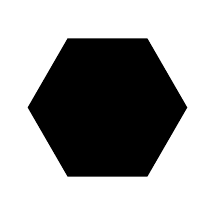
\begin{tikzpicture}[x=0.35in, y=0.35in]
				\begin{scope}[yshift=0]
        \fill[black] (0:1.14) \foreach \x in {60,120,...,359} {
                -- (\x:1.14)
            }-- cycle (90:1.14);
            \end{scope}
			\end{tikzpicture}
			\caption{External hex}
		\end{subfigure}\begin{subfigure}[b]{.15\linewidth}
			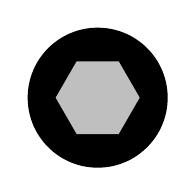
\begin{tikzpicture}[x=0.35in, y=0.35in]
				\begin{scope}[yshift=0]
				\fill[black] (0,0) circle (1);
        \fill[lightgray] (0:0.6) \foreach \x in {60,120,...,359} {
                -- (\x:0.6)
            }-- cycle (90:0.6);
            \end{scope}
			\end{tikzpicture}
			\caption{Socket hex}
		\end{subfigure}\begin{subfigure}[b]{.15\linewidth}
			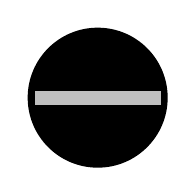
\begin{tikzpicture}[x=0.35in, y=0.35in]
				\begin{scope}[yshift=0]
				\fill[black] (0,0) circle (1);
       			\fill[lightgray] (-0.9,-0.1)--(0.9,-0.1)--(0.9,0.1)--(-0.9,0.1)--cycle;
            \end{scope}
			\end{tikzpicture}
			\caption{Flathead}
		\end{subfigure}\begin{subfigure}[b]{.15\linewidth}
			
\begin{tikzpicture}[x=0.35in, y=0.35in]
				\begin{scope}[yshift=0]
				\fill[black] (0,0) circle (1);
	        	\fill[lightgray] (-.8,-.1) arc (90:0:0.7) -- (0.1,-0.8) arc (180:90:0.7) -- (0.8,0.1) arc (270:180:0.7) -- (-0.1,0.8) arc (360:270:0.7) -- cycle;
	        	
	        	\fill[gray] (-.35,-.05) arc (90:0:0.3) -- (0.05,-0.35) arc (180:90:0.3) -- (0.35,0.05) arc (270:180:0.3) -- (-0.05,0.35) arc (360:270:0.3) -- cycle;
            \end{scope}
			\end{tikzpicture}
			\caption{Phillips}
		\end{subfigure}\begin{subfigure}[b]{.15\linewidth}
			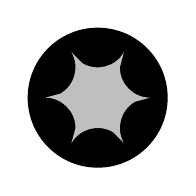
\begin{tikzpicture}[x=0.35in, y=0.35in]
				\begin{scope}[yshift=0]
				\fill[black] (0,0) circle (1);
	        	\fill[lightgray] (0.75,0) \foreach \x in {0,60,...,359} {
                	-- ({0.75*cos(\x}, {0.75*sin(\x)}) arc ({270+\x}:{180+\x}:{0.75*tan(30)})
            	} -- cycle;
            \end{scope}
			\end{tikzpicture}
			\caption{Torx}
		\end{subfigure}\begin{subfigure}[b]{.15\linewidth}
			
\begin{tikzpicture}[x=0.35in, y=0.35in]
				\begin{scope}[yshift=0]
				\fill[black] (0,0) circle (1);
       			\fill[lightgray] (-0.4,-0.4)--(0.4,-0.4)--(0.4,0.4)--(-0.4,0.4)--cycle;
            \end{scope}
			\end{tikzpicture}
			\caption{Robertson}
		\end{subfigure}
		\caption{Common drive types on engineering fasteners.}
	\end{figure}
	
	\index{screws and bolts!heads}
	\begin{asparaenum}[a)]
		\item \textit{External hex} is very robust, although preferred only when side access is available as it has a large profile.
		\item \textit{Socket hex} has become an industry preferred head, very easy to access from head-on or in a deep pocket.
		\item \textit{Flathead} is not a preferred drive type; it is very easy to have driver fall out while using, and the torque-transferring capacity is quite low.
		\item \textit{Phillips} heads are very much not preferred as they are very easy to cam out (in fact, they were designed to do so as a means of limiting the installation torque). When driving a Phillips screw, apply inward pressure, and make sure the proper size driver is selected (it should fit nicely).
		\item \textit{Torx} is a preferred drive method, but more expensive and the tools to use it are less common. Very difficult to strip out. When using button-head or flat-head screws, if a Torx variant is available, it can be wise to opt for it as the torque-transferring capacity is higher.
		\item \textit{Robertson} or square drive is somewhat preferred, but not common. It is usually found only in wood screws.
	\end{asparaenum}
	
	The drive heads on flat head, button head, and shoulder screws are necessarily smaller than those of socket head screws, and thusly strip out easier.
	
	\index{screws and bolts!preload}
	\begin{figure}[H]
		\includegraphics[width=0.5\textwidth]{imgs/bolt_preload.png}
		\caption{Aspects of a bolted joint.}
		 \label{fig:bolted_joint} 
	\end{figure}
	
	When you tighten a screw to a torque, this not only prevents the nut from falling off, but clamps the parts together. This clamping force that is imparted upon installation is \textit{preload}\index{preload}, which is very important in threaded joints. For shear loads as illustrated in Figure \ref{fig:bolted_joint}, the load is best carried by the friction inbetween plates rather than shearing the pin itself, since the load is distributed across a larger area. For joints that seal against pressures, preload is imperative as it prevents separation under pressure.
	
	\index{thread!pitch}
	The preload depends both on how much torque is applied to the fastener, and the pitch of the thread. A finer-pitched screw will impart greater preload. Finer-pitched screws also have the benefit of an increased core (minor) diameter, so greater strength in shear. The finer threads may be more fragile and require tighter tolerance, though.
	
	Spreading the load across the greater area increases rigidity and decreases backlash, egg-out, and strength. However, too much torque can dig the head of the bolt/screw into the underlying material, especially if it is soft (like plastic, or even aluminum). As such, care not to overtorque, or a washer may be needed.
	\index{washers}
	\begin{figure}[H]
		\centering
		\begin{subfigure}[b]{.24\linewidth}
			\includegraphics[width=0.7\textwidth]{imgs/plainwasher.png}
			\caption{Plain washer}
		\end{subfigure}\begin{subfigure}[b]{.24\linewidth}
			\includegraphics[width=0.7\textwidth]{imgs/machinewasher.png}
			\caption{Machine washer}
		\end{subfigure}\begin{subfigure}[b]{.24\linewidth}
			\includegraphics[width=0.7\textwidth]{imgs/fenderwasher.png}
			\caption{Fender washer}
		\end{subfigure}
		\caption{Plain washers of differring sizes}
	\end{figure}
	
	\index{threads!threaded inserts}
	
	Bolts thread into nuts, which can be replaced if they strip out. But if the material a screw threads into strips, then that whole piece will need to be replaced or repaired- which can be even more costly. There are some considerations that can be made to ensure success when using integral threads. The first is to make sure to use coarse (not fine) threads in soft materials like aluminum or plastic. Another option is to use thread inserts.
	
	\begin{figure}[H]
		\centering
		\begin{subfigure}[b]{.24\linewidth}
			\includegraphics[width=0.5\textwidth]{imgs/helicoil.png}
			\caption{Helicoil}
		\end{subfigure}\begin{subfigure}[b]{.24\linewidth}
			\includegraphics[width=0.5\textwidth]{imgs/tanglock.png}
			\caption{Tang-lock insert}
		\end{subfigure}\begin{subfigure}[b]{.24\linewidth}
			\includegraphics[width=0.5\textwidth]{imgs/rivnut.png}
			\caption{Rivnut}
		\end{subfigure}\begin{subfigure}[b]{.24\linewidth}
			\includegraphics[width=0.5\textwidth]{imgs/pemnut.png}
			\caption{PEM nut}
		\end{subfigure}
		
		\begin{subfigure}[b]{.24\linewidth}
			\includegraphics[width=0.5\textwidth]{imgs/heatset.png}
			\caption{Heat-set insert}
		\end{subfigure}\begin{subfigure}[b]{.24\linewidth}
			\includegraphics[width=0.5\textwidth]{imgs/teenut.png}
			\caption{Tee nut}
		\end{subfigure}\begin{subfigure}[b]{.24\linewidth}
			\includegraphics[width=0.5\textwidth]{imgs/woodsti.png}
			\caption{Wood tapping insert}
		\end{subfigure}
		\caption{Various threaded inserts}
	\end{figure}
	
	\begin{asparaenum}[a)]
		\item \textit{Helicoils} can be installed after a thread strips out, or before it does preventatively. They are a coiled piece of metal formed like threads.
		\item \textit{Tang-lock inserts} work much like helicoils, but are solid-bodied rather than coiled, and have locking tangs that can be hammered down on installation to make sure the insert doesn't back out.
		\item \textit{Rivnuts} (rivet nuts) can be installed into holes in thin metal to provide ample threads for fastening. They work much like rivets (more on those later), but need a special tool.
		\item \textit{PEM nuts} serve the same purpose as rivnuts, but are simply pressed into the sheet they are to be installed in.
		\item \textit{Heat-set inserts} are for plastic. They are installed by heating them up with a soldering iron and pressing them into thermoplastic. An excellent addition to 3D prints. \index{3D printing!heat-set inserts}
		\item \textit{Tee nuts} are meant to be pressed into wood, much like a PEM nut. The large flange prevents tear-out and helps distribute load in soft wood.
		\item \textit{Wood tapping inserts} are much like tang-lock inserts, but with larger wings suitable for wood.
	\end{asparaenum}
	
	Threaded joints have one big weakness, and that is their subsceptibility to vibration. There are many solutions to try and combat this.
	\index{threads!locking}
	\index{positive retention}
	\begin{figure}[H]
		\centering
		\begin{subfigure}[b]{.24\linewidth}
			\includegraphics[width=0.8\textwidth]{imgs/lockwire.png}
			\caption{Safety/lock wire}
		\end{subfigure}\begin{subfigure}[b]{.24\linewidth}
			\includegraphics[width=0.8\textwidth]{imgs/threadlocker.jpeg}
			\caption{Threadlocker}
		\end{subfigure}\begin{subfigure}[b]{.24\linewidth}
			\includegraphics[width=0.5\textwidth]{imgs/nylock.png}
			\caption{Nylock nut}
		\end{subfigure}\begin{subfigure}[b]{.24\linewidth}
			\includegraphics[width=0.7\textwidth]{imgs/kaynut.png}
			\caption{Kay/jet nut}
		\end{subfigure}
		
		\begin{subfigure}[b]{.24\linewidth}
			\includegraphics[width=0.5\textwidth]{imgs/jamnut.png}
			\caption{Jam nut}
		\end{subfigure}\begin{subfigure}[b]{.24\linewidth}
			\includegraphics[width=0.5\textwidth]{imgs/nordlock.png}
			\caption{Nordlock washer}
		\end{subfigure}\begin{subfigure}[b]{.24\linewidth}
			\includegraphics[width=0.5\textwidth]{imgs/splitlock.png}
			\caption{Split lock washer}
		\end{subfigure}\begin{subfigure}[b]{.24\linewidth}
			\includegraphics[width=0.5\textwidth]{imgs/castlenut.png}
			\caption{Castle nut}
		\end{subfigure}
		\caption{Thread locking strategies.}
	\end{figure}
	
	\begin{asparaenum}[a)]
		\item \textit{Lock wire} requires tedious installation and bolts with cross-drilled holes to feed the stainless steel wire through. That said, when it is installed properly, it is virtually failure-proof, and as such is the standard in many aerospace and motorsport applications. 
		\item \textit{Threadlocker} (sometimes referred to by the brand name Loctite) comes in various different strengths and can be used on metal-on-metal contact. It's basically long-cure, specially formulated superglue. However, it does attack many plastics, so be careful! It also requires time to cure to full strength and so is not an instant fix, but must be premeditated.
		\item \textit{Nylock nuts} have a nylon patch that deforms when the threads pass through it. The nut should be installed metal-side first, nylon-side last. These are limited use ($<$50 uses).
		\item \textit{Kay/Jet nuts} (metal locknuts) work on the same idea as nylock nuts, but in this case, the nut is deformed and interferes with the thread. It is quite difficult to thread into these nuts. These are extremely limited use ($<$5 uses) but will work in extreme temperatures, unlike nylock nuts.
		\item \textit{Jam nuts} are simply a second nut jammed up against the first nut. This enables easy adjustment, but is not a very positive way of locking something in place.
		\item \textit{Nordlock washers} are special ratcheting washers which prevent loosening when properly torqued. There are many different types of locking washers.
		\item \textit{Split lock washers} are cheap washers which arguably do not actually prevent loosening.
		\item \textit{Castle nuts} are nuts with slots through which a pin can be fed, locking the nut to the bolt it is secured to. A very robust method.
	\end{asparaenum}
	
	\subsection{Rivets}
	\index{rivets}	
	Pop rivets are a light and cheap method of fastening. However, they require a special gun and are one-time use. They must be drilled out in order to remove them. They are weaker than bolts, so more must be used, but overall, they are a lighter option. Installation is also more picky than bolting. However, they can still be a time-saver over bolts when disassembly is not a factor.
	
	Rivets are specified by diameter and \textit{grip length} - the amount of material sandwiched together that they can grip. Rivets should be installed straight to close-fit holes with the plates already pulled together.
	
	\begin{figure}[H] \centering
		\includegraphics[width=0.9\textwidth]{imgs/rivet_install.jpeg}
		\caption{Left: Process of Rivet Installation. Right: Diagnosing rivet failures.}
	\end{figure}
	
	Hot rivets are a very different animal than pop rivets. These require very specialized equipment, and work by heating up a rivet to molten temperature, inserting it through the hole to be secured, and hammering it so it expands and mushrooms out on both sides. As the rivet cools, it shrinks further, creating an incredibly robust and secure connection.	
	
	\subsection{Shaft Retention}
	\index{snap rings, e-clips, circlips}
	Retaining rings are used to constrain objects along a shaft.
	
	\begin{figure}[H]
		\centering
		\includegraphics[width=0.45\textwidth]{imgs/shaft_snapringgroove.png}
		\includegraphics[width=0.45\textwidth]{imgs/snapringtool.jpeg}
		\caption{Left: Shaft with groove for retaining ring. Right: Snap ring pliers.}
	\end{figure}
	
	\begin{figure}[H]
		\centering
		\begin{subfigure}[b]{.24\linewidth}
			\includegraphics[width=0.6\textwidth]{imgs/shaftcollar.png}
			\caption{Shaft collar}
		\end{subfigure}
		\begin{subfigure}[b]{.24\linewidth}
			\includegraphics[width=0.7\textwidth]{imgs/pushonring.png}
			\caption{Push-on ring}
		\end{subfigure}
		\begin{subfigure}[b]{.24\linewidth}
			\includegraphics[width=0.7\textwidth]{imgs/eclip.png}
			\caption{E-clip}
		\end{subfigure}
		\begin{subfigure}[b]{.24\linewidth}
			\includegraphics[width=0.7\textwidth]{imgs/ext_snapring.png}
			\caption{External snap ring}
		\end{subfigure}
		\begin{subfigure}[b]{.24\linewidth}
			\includegraphics[width=0.7\textwidth]{imgs/int_snapring.png}
			\caption{Internal snap ring}
		\end{subfigure}
		\begin{subfigure}[b]{.24\linewidth}
			\includegraphics[width=0.7\textwidth]{imgs/spiralring.png}
			\caption{Spiral ring}
		\end{subfigure}\begin{subfigure}[b]{.24\linewidth}
			\includegraphics[width=0.7\textwidth]{imgs/circlip.png}
			\caption{Circlip}
		\end{subfigure}
		\caption{Shaft Retaining Technologies}
	\end{figure}
	
	
	\begin{asparaenum}[a)]
		\item \textit{Shaft collars} are heavy and high-profile, but easily removable and adjustable. They come in different bore shapes (hex, round, keyed, etc) and in one or two-piece varieties.
		\item \textit{Push-on rings} are pushed onto shafts (no groove needed) and ideally ratchet on, never coming off.
		\item \textit{E-clips} can be pushed radially into a groove. They are aided by the use of a snap-ring tool to splay them apart, but it is not necessary. They can be installed without passing the clip over the end of a shaft.
		\item \textit{External snap rings} are expanded by a snap-ring tool, and installed over the groove of a shaft.
		\item \textit{Internal snap rings} are compressed by a snap-ring tool, and installed into the groove of a housing.
		\item \textit{Spiral rings} are wound into grooves. They're annoying and rare.
		\item \textit{Circlips} are very stiff, low-profile retaining clips intended for permanent installation.

	\end{asparaenum}
	
	When working with expanding rings, it is very important to not over-extend them on installation. It is very easy to over-extend and damage the rings -leading to successful installation, but potential for the ring to fall off later during use - if expanded much more than is necessary to feed them over the shaft.
	
	\subsection{Adhesives}
	\index{adhesives!epoxies, superglue, tape}
	\index{hook-and-loop}
	
	\begin{asparaenum}[a)]
		\item \textit{Retaining compound} such as Loctite Green is meant to bond bearings to their housings.
		\item \textit{Epoxies} are two-part adhesives that are mixed immediately prior to application. They can cure quickly.
		\item \textit{Cyanoacrylate/superglue} adhesives are good for many plastics. Loctite has a good design/test guide for different plastic/glue combinations.
		\item \textit{Tapes} can be quite useful. Good duct tape and gaffer's tape can be used for high-fidelity prototyping and quick fixes.
		\item \textit{Pressure-sensitive tape} such as 3M VHB can be incredibly strong. Follow the manufacturer's directions for maximum strength.
		\item \textit{Hook-and-loop tape} and dual-lock can produce easy but secure removable components.
	\end{asparaenum}
	
	
	\subsection{Panel Fasteners}
	\index{panel fasteners}
	Often panels need to attached to protect something, provide a clean cosmetic appearance, or smooth over a gap for aerodynamic purposes, while still providing easy service to the underlying components. There are a few solutions to this which are more robust and positive than Velcro (which may be perfectly acceptable in many cases). These solutions make sure that the fasteners are kept with the panel so there's no scrambling around to find the panel.
	
	\begin{figure}[H]
		\begin{subfigure}[b]{.35\linewidth}
			\includegraphics[width=0.9\textwidth]{imgs/dzus_tabs.jpeg}
			\caption{Dzus tabs}
		\end{subfigure}
		\begin{subfigure}[b]{.3\linewidth}
			\includegraphics[width=0.6\textwidth]{imgs/pushpull_panel_screw.png}
			\caption{Push-pull panel pin}
		\end{subfigure}
		\begin{subfigure}[b]{.3\linewidth}
			\includegraphics[width=0.6\textwidth]{imgs/panel_screw.png}
			\caption{Captive panel screw}
		\end{subfigure}
	\end{figure}
	
	\begin{asparaenum}[a)]
		\item \textit{Quarter turn fasteners} such as \textit{Dzus tabs} are an easily removable, robust solution. Some require a simple tool (flat-blade screwdriver) to remove. Often found in motorsport applications, they are permanently installed into both the frame and panel. They stick out a very small amount - the thickness of the tab.
		\item \textit{Push-pull panel pins}, like \href{https://www.mcmaster.com/panel-fasteners/screws-and-bolts/push-pull-captive-panel-screws/}{\color{red}\underline{these on McMaster-Carr}} are a light-duty solution, but do not require any special machining to integrate, just drill holes of the right diameters. They also do not require any special tools to remove or attach, and stay captive with the panel they are attached to. However, they do stick out from the panel quite significantly.
		\item \textit{Captive panel screws} are effectively screws that are kept captive to the panel. Like any screw, they require the appropriate tool to remove.
	\end{asparaenum}
	
	\subsection{The Zip Tie}
	\index{zip tie}
	I had to save the best for last: the \textit{zip tie}, or \textit{cable tie}. Zip ties have a slight reputation as a hackish solution, but this is more a result of people overusing them or overestimating how much they can accomplish. That being said, they can do a lot, from their intended use of holding bundles of wires together, to forming agitating flappers on ball feeding mechanisms. Zip ties come in different materials, although the most common is nylon.
	
	\begin{figure}[H]
		\includegraphics[width=0.9\textwidth]{imgs/ziptie.png}
		\caption{The zip tie.}
	\end{figure}
	
	These have a head attached to a long strip, which can be fed into the head to form a loop. The head is ratcheting, so when the tail is pulled through, it will not loosen (until it breaks). Multiple zip ties can be chained together to form a longer one. Some special zip ties can be reused - they have a release lever.

	\section{Fabrication Paradigms / Traditions}
	To draw an analogy to cuisine... up to this point we've talked about different ingredients - the different herbs, meats, vegetables, fruits, grains that you might use in a kitchen to make a dish with. You can combine them in a lot of different ways, but there are some combinations that make more sense than others, and some that have become traditional because of this. That isn't to say that you can't mix and match and add as you see fit - or even start your own tradition - but there are combinations of technologies that are more common than others. 
	
	\subsection{The 80/20 Tradition}
	\index{extrusions:t-slot framing}
	One common tradition is that of using t-slot framing as introduced in section \ref{subsec:extrusions}. There are many different components that can be used with t-slot framing. This tradition is quite deep and even has sub-traditions.
	
	\begin{figure}[H]
	\begin{subfigure}[b]{.32\linewidth}
		\includegraphics[width=0.9\textwidth]{imgs/tradition_8020_tnut.jpeg}
		\caption{T nut}
	\end{subfigure}\begin{subfigure}[b]{.32\linewidth}
		\includegraphics[width=0.9\textwidth]{imgs/tradition_8020_ext_plate.jpeg}
		\caption{Joiner plate}
	\end{subfigure}\begin{subfigure}[b]{.32\linewidth}
		\includegraphics[width=0.9\textwidth]{imgs/tradition_8020_ext_bracket.jpeg}
		\caption{External bracket}
	\end{subfigure}
	
	\begin{subfigure}[b]{.55\linewidth}
		\includegraphics[width=0.9\textwidth]{imgs/tradition_8020_anchor.jpeg}
		\caption{Anchor fastener}
	\end{subfigure}\begin{subfigure}[b]{.4\linewidth}
		\includegraphics[width=0.9\textwidth]{imgs/tradition_8020_corner.png}
		\caption{Corner block}
	\end{subfigure}
	\caption{Key components in the 80/20 tradition.}
	\end{figure}
	
	\begin{asparaenum}[a)]
		\item \textit{T nuts} are the basic ingredient of the 80/20 tradition. They come in many flavors: some can be dropped in to a t-slot, some can be rolled in, some can only be slid in through the end. However, they all serve the same purpose: they're a nut that stays captive in the T-slot.
		\item \textit{Joiner plates} are one way of securing tubes to other tubes. They're straightforward, and come in many sizes.
		\item \textit{External brackets} are another way of securing tubes to other tubes. These come in many sizes and thicknesses, sometimes with a reinforcing strip (as shown).
		\item \textit{Anchor fasteners} (sometimes nicknamed \textit{lollipop connectors}) are one type of end connector. There are many types of end connectors but these seem to be the most common. The framing gets milled out to accept the round portion of the connector. The connector then fits into one frame, and a bolt going through that connector gets tightened into a t nut inside another frame. The heads of the bolts can be quite frustrating to access and tighten down perfectly, and these also require that the ends of the tubes get milled perfectly square.
		\item \textit{Corner blocks} allow corners to get joined together in a very clean fashion. The ends of the extrusions must be tapped to accept a bolt. It is possible to make printed versions of these that allow extrusions to come together at odd angles.
	\end{asparaenum}
	
	Overall, 80/20 is a very flexible paradigm, but quite heavy and expensive, and can be prone to loosening and sliding under vibration.
	
	\subsection{The Sheet metal Tradition}
	\index{sheet metal}
	\index{rivets}	
	Airplanes have pioneered this method of cut and folded sheet metal, riveted together to make complex structures. It's a somewhat like industrial origami.
	
	\begin{figure}[H]
		\includegraphics[width=0.8\textwidth]{imgs/tradition_sheetmetal_148.png}
		\caption{An FRC (FIRST Robotics Competition) chassis made from riveted sheet metal.}
	\end{figure}
	
	Sheet metal can be extremely light, as it has the capability to put material where it is needed most. It is necessary that the sheet be bent to add out-of-plane stiffness. Sheet metal is one of the cheapest forms of metal, pound-for-pound, although the cutting required to make these frames usually produces a considerable amount of waste stock. 
	
	Sheet metal is a very scalable process in mass quantity, which is why many things are made from it, even if they aren't riveted as well.
	
	Rivets work best in shear and with plenty of redundancy. Bolts can also be used, but they will tend to egg out the holes, so the sheet metal itself becomes the limiting factor, making the use of a higher quantity of rivets the stronger choice.
	
	\href{https://johnvneun.com/blog/2020/4/4/sheetmetal-design}{\color{red}\underline{John V Neun}} has some examples of how to use sheetmetal.
	
	\subsection{The Fingerjointed Plate Tradition}
	What do you do if you have a way of cutting plates, but no bender? Well, cut thicker ones, and use finger joints to stick it all together! Woodworkers have long used finger joints to make nice craftwork using glue and nail. But if you want to quickly build something and maybe tear it apart, gluing or nailing aren't a good proposition.
	
	\begin{figure}[H]
		\includegraphics[width=0.55\textwidth]{imgs/tradition_fingerjoint.png}
		\includegraphics[width=0.4\textwidth]{imgs/fingerjoint_battlebot.png}
		\caption{Fingerjointed and bolted assemblies.}
	\end{figure}
	
	Such joints are popular among the hobbyist community, and often feature captive nuts and bolting shown above to help keep things together. The fingers transmit shear load, while the bolts help keep things together. The joint above on the left would still flex quite a bit almost like a hinge, so putting another plate perpendicular to both - making a box or gusset - would help the structural integrity more.
	
	These joints can also be made with metal, or at odd angles.
	
	\subsection{The Bracket and Tube Tradition}
	\index{extrusions}	\index{tube}
	Sheet metal is cool, but doesn't have to be used that much. It isn't a very effective way at spanning long distances, and requires lead time since you have to get the profile cutting supplier/equipment to do it.
	
	\begin{figure}[H]
		\includegraphics[width=0.6\textwidth]{imgs/tradition_gussetbox.jpeg}
		\caption{Tubes held together with sheet metal gussets.}
	\end{figure}
	
	Brackets can come in many shapes and sizes and purposes. They can join together tubes by sandwiching them (see the hypotenuse), join tubes by being installed to the side (see the joint of the legs), or mount extra components like bearings and motors. Brackets are cheap, often made of sheet metal and produced in large quantities, as is box tube. You can even purchase or make extrusion with regularly drilled holes, so that you don't need to bother fabricating holes into the tubes come time to build a structure.
	
	As with sheet metal, both bolts and rivets can be used - but the use of redundant rivets rather than bolts can end up being lighter and stronger, although less serviceable. \index{rivets}
	
	\subsection{The Spaceframe Tradition}
	\index{extrusions}
	\index{welding}
	\index{tube}	
	Tubes are strong and light. Welds are even lighter than gussets. Welding tubes together directly and using round, rather than square tube to prevent stress concentrators creates \textit{spaceframes}\index{spaceframe} or \textit{tubeframes}\index{tubeframe}.
	
	% Is chunky a tradition? I can't think of any examples... it's kinda just a thing that happens
	
	\begin{figure}[H]
		\includegraphics[width=0.8\textwidth]{imgs/tradition_tubeframe.jpeg}
		\caption{A spaceframe for a Formula SAE racecar.}
	\end{figure}
	
	Spaceframes are time-consuming to produce, as tubes must be cut to length and have the ends shaped so they fit together, a process known as \textit{coping}\index{coping} or \textit{notching}\index{notching}. Additionally, a jig or figure is required to hold all of the tubes in place before they are welded. On the upside, they allow for near-ultimate flexibility in material placement and routing.
	
	\begin{figure}[H]
		\includegraphics[width=0.8\textwidth]{imgs/tradition_tubeframe_jigging.jpeg}
		\caption{A jig for a spaceframe.}
	\end{figure}